% pdf version
\documentclass[12pt,a4paper]{settings/ugent-doc}
\geometry{bottom=2.5cm,top=2.5cm,left=2.5cm,right=2.5cm} 

\renewcommand{\baselinestretch}{1.15}

\usepackage{fontspec}
\setmainfont[ExternalLocation=fonts/]{SourceSerifPro-Light.ttf}
[ItalicFont=SourceSerifPro-LightItalic.ttf,
BoldFont=SourceSerifPro-Regular.ttf,
BoldItalicFont=SourceSerifPro-Italic.ttf]

\setsansfont[ExternalLocation=fonts/]{WorkSans-Regular.ttf}
[BoldFont=WorkSans-Medium.ttf]

\usepackage[main=english,french,dutch]{babel}
% \usepackage{libertine}
% \usepackage{libertinust1math}
\usepackage{amsmath} % math equations

% code snippets
\setmonofont[ExternalLocation=fonts/]{SourceCodePro-Regular.ttf}
[ItalicFont=SourceCodePro-Italic.ttf,
BoldFont=SourceCodePro-SemiBold.ttf]

\usepackage{listings}

% transcriptions:
\usepackage{xparse}
\usepackage{enumitem}

% acronyms
\usepackage[printonlyused,withpage]{acronym}

% figures
\usepackage{graphicx} 
\usepackage{changepage}
\usepackage{pgfplots}
\graphicspath{{./figures/}}

% Bibliography
\usepackage[backend=biber, style=apa, sorting=nyt, hyperref=true]{biblatex} 
\addbibresource{references.bib}
\usepackage{csquotes} % Suggested when using babel+biblatex

% Ugent specific
\usepackage[colorlinks=true, allcolors=ugentblue]{hyperref} % Hyperreferences
\usepackage[parfill]{parskip} % Whitespace between paragraphs and no indentation

% code snippets
\usepackage{listings}
\usepackage{minted}
\usepackage{caption}
\usepackage{dirtree}
\captionsetup{justification=centering, margin=2cm}
\definecolor{mygray}{rgb}{0.95, 0.95, 0.95}
\definecolor{codeBlue}{rgb}{0.16, 0.22, 0.69}
\definecolor{codeGreen}{rgb}{0.16, 0.6, 0.44}
\setminted{
  breaklines=true,
  breakanywhere=true,
  fontsize=\footnotesize,
  bgcolor={mygray},
  style=lovelace
}
\makeatletter
\def\dontdofcolorbox{\renewcommand\fcolorbox[4][]{##4}}
\makeatother
\dontdofcolorbox

% styling table of contents
% \setcounter{tocdepth}{4}
\setcounter{secnumdepth}{4}

% hbox warning margin
\hfuzz=2pt

% for diagrams using Mathcha
\usepackage{tikz}
\usepackage{pgf-umlsd}
\usepgflibrary{arrows} % for pgf-uml

% for diagrams using svg
% \usepackage{svg} -> manual conversion to pdf using inkscape
% -> use \includegraphics{... .pdf}

% for tables
\usepackage{booktabs}

% for footnotes
\counterwithout{footnote}{chapter}

% for links
\usepackage{hyperref}

% extended abstract
\usepackage{multicol}
\setlength{\columnsep}{5mm}
\usepackage{lipsum}

% titel blad
\usepackage{pdfpages}

% ---------------------------------------------

\thesubtitle{Linked Data}
\usepackage{ulem} % for colored underline
\renewcommand{\ULthickness}{2pt} % adjust thickness of underline
\thetitle{\uline{\color{ugentblue} Pre-culling geometric linked building data\\ for lightweight viewers}}
\infoboxa{Master's dissertation submitted in order to obtain the academic degree of \\
Master of Science in de ingenieurswetenschappen: architectuur
}
\infoboxb{Supervisor:
\begin{tabular}[t]{lll}
    Prof.\ ir.-arch.\ Paulus Present\\ % note syntax 'short space'
\end{tabular}
}
\infoboxc{Counselors: 
\begin{tabular}[t]{lll}
    Ir.-arch.\ Jeroen Werbrouck\\ % note syntax 'short space'
    Prof.\ dr.\ ir.\ arch.\ Ruben Verstraeten
\end{tabular}
}

\infoboxd{Philippe Soubrier 01702837 philippe.soubrier@ugent.be}
\infoboxe{Academic year: 2022--2023}

% ---------------------------------------------
\begin{document}
% 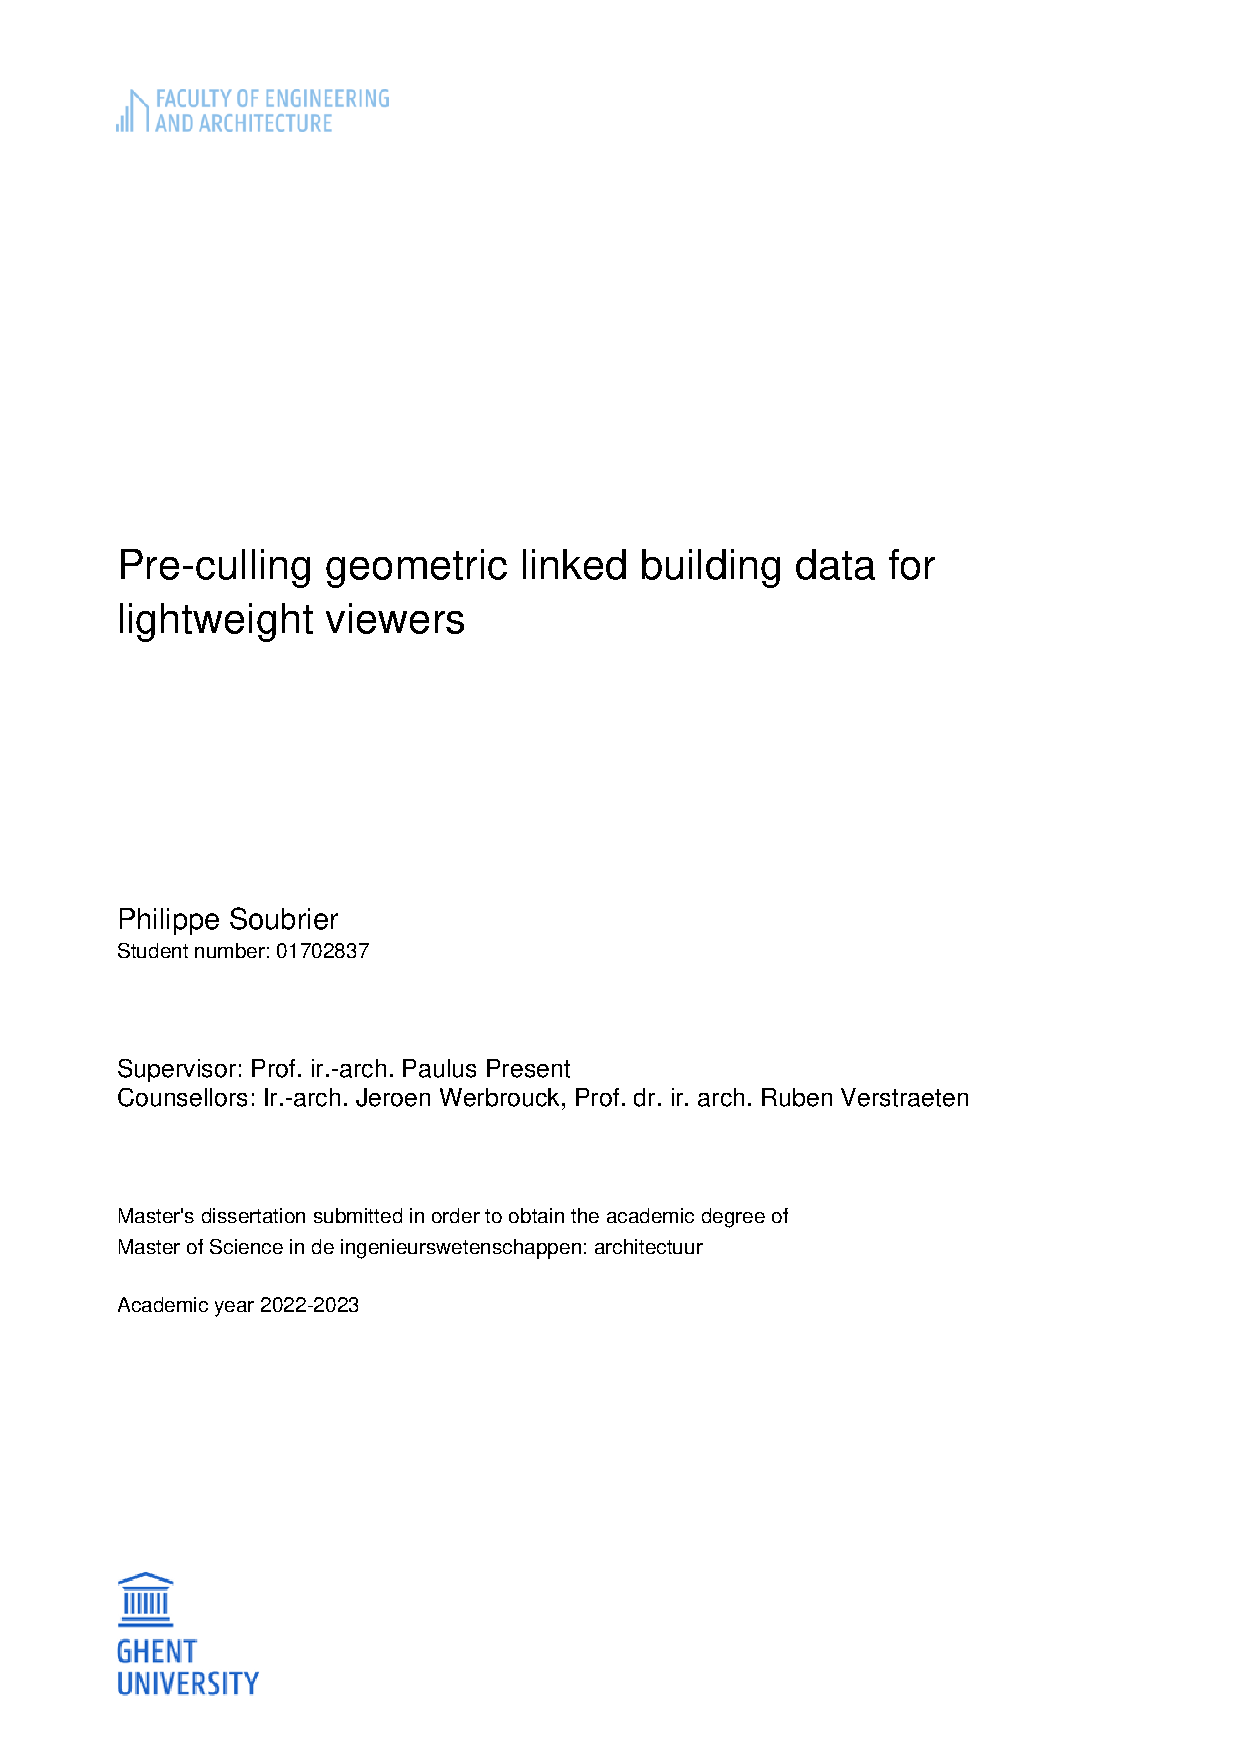
\includepdf[pages={1}]{chapters/pre/titelblad.pdf}
\maketitle
\normalem
\counterwithin{listing}{chapter}
\hspace{6cm}
\pagenumbering{alph}

De auteur(s) geeft (geven) de toelating om deze masterproef voor consultatie
beschikbaar te stellen en delen van de masterproef te kopiëren voor persoonlijk
gebruik.

Elk ander gebruik valt onder de bepalingen van het auteursrecht, in het bijzonder met
betrekking tot de verplichting de bron uitdrukkelijk te vermelden bij het aanhalen van
resultaten uit deze masterproef.

\vspace{1cm}

The author(s) gives (give) permission to make this master dissertation available for
consultation and to copy parts of this master dissertation for personal use.

In all cases of other use, the copyright terms have to be respected, in particular with
regard to the obligation to state explicitly the source when quoting results from this
master dissertation.

\vspace{2cm}
\begin{flushright}
  Philippe Soubrier\\
  Ghent, 25 May 2023
\end{flushright}

\vfill

Deze masterproef vormt een onderdeel van een examen. Eventuele opmerkingen die door de beoordelingscommissie tijdens de mondelinge uiteenzetting van de masterproef werden geformuleerd, werden niet verwerkt in deze tekst.

This master's dissertation is part of an exam. Any comments formulated by the assessment committee during the oral presentation of the master's dissertation are not included in this text.
{\huge\sffamily{Preface}}

This thesis is the result of research about \ac{ar} in the \ac{aec} sector and the use of linked data to improve the performance of \ac{ar} applications. It evolved into a broader research about lightweight viewers with the same need for performance improvements. It would not have been possible without the help and guidance of several people, whom I would like to thank.

Firstly, I would like to thank my supervisor Paulus Present and counselors Jeroen Werbrouck and Professor Ruben Verstraeten for their guidance, feedback, and discussions we had throughout the entire process. In particular, I would like to thank Jeroen Werbrouck for his previous courses that sparked my interest in the domain of coding and web development, and for his valuable feedback on the technical aspects of this thesis.

Secondly, I would like to thank Professor Tiemen Strobbe for taking the time to explain the workings of the Qonic viewer, which inspired the developed framework of this thesis. Finally, I would like to thank Hanne den Biesen and Bram van Rooijen for thoroughly proofreading this thesis. Their feedback and comments were invaluable and I am very grateful for their help.
\acresetall % reset acronyms
\begin{center}
    \sffamily
    \huge Pre-culling geometric linked building data
    for lightweight viewers

    \Large Philippe Soubrier

    \normalsize
    Supervisor: Prof.\ ir.-arch.\ Paulus Present         \\
    Counselors: Ir.-arch.\ Jeroen Werbrouck \\
    Prof.\ dr.\ ir.\ arch.\ Ruben Verstraeten
\end{center}

Master’s dissertation submitted in order to obtain the academic degree of \\
Master of Science in de ingenieurswetenschappen: architectuur

Academic year 2022-2023
\section*{\LARGE Abstract}
\lipsum[1-2]

\vfill
\emph{Keywords} \textbf{
    - BIM, Linked Data, Culling, 3D viewers, Web-app
}
\vspace{1cm}
\acresetall

\newgeometry{bottom=2cm,top=2cm,left=1.5cm,right=1.5cm}
\newgeometry{bottom=2cm,top=2cm,left=1.5cm,right=1.5cm}
\begin{center}
    \sffamily
    \huge Extended Abstract

    \Large Philippe Soubrier

    \normalsize
    Supervisor: Prof.\ ir.-arch.\ Paulus Present\\
    Counselors: Ir.-arch.\ Jeroen Werbrouck, Prof.\ dr.\ ir.\ arch.\ Ruben Verstraeten
\end{center}
\begin{refsection}
    \defbibheading{bibliography}[]{}
    \begin{multicols}{2}
        \small
        \emph{Abstract} \textbf{
            - This thesis tackles the issue of visualizing complex \ac{bim} models on resource-limited devices in the \ac{aec} sector, introducing \enquote{pre-culling} to reduce the 3D scene to the viewer's view frustum. By utilizing Semantic Web technologies like the \ac{rdf} and the \ac{sparql}, \ac{bim} models are stored and queried as databases, thereby facilitating their segmentation.
        }

        \emph{Keywords} \textbf{
            - Linked Data, lightweight viewers, culling, BIM, SPARQL
        }
    
        The \ac{aec} industry has undergone significant technological transformations over the past few decades. The advent of 3D modeling constituted a major shift in the industry, heralding a new era of geometric data representation. The subsequent introduction of \ac{bim} has functioned as a versatile repository for semantics derived from various applications throughout the design and construction processes, including but not limited to cost estimation, energy analysis, and production planning. However, as \cite{Werbrouck2018} highlighted, the next challenge for the \ac{aec} industry is related to the domain-specific nature of current \ac{bim} software solutions, which remain inaccessible to other disciplines. This data \textbf{management} issue is currently being tackled by entities such as the \ac{lbd-cg} and academic institutions like the University of Ghent, leveraging the potential of Semantic Web technologies for more integrated and efficient data handling, thereby enabling interdisciplinary collaboration. The term \ac{ldbim} is used in this thesis to denote this emerging milestone.

        Alongside this evolution, in tandem with the increasing amount of semantic data, the geometric data describing a \ac{bim} model is also growing in size and complexity. This makes the task of visualization increasingly complex on newer, resource-limited devices used in the industry. Such devices, for example, smartphones and tablets, are becoming increasingly popular on construction sites. Existing solutions use a filtering step in the visualization process, known as culling. This computational step necessitates the processing of the entire 3D file or scene to cull it to the viewer's view frustum \parencite{Johansson2015}. This operation produces a minimal 3D scene, which is then utilized for the significantly more resource-intensive process of rendering.

        A bottleneck arises when the initial 3D scene, upon which the in-viewer culling process is performed, becomes too large for the device to handle. As a solution to this problem, this thesis proposes the use of a \textbf{pre-culling} step. In this process, and with the aid of Semantic Web technologies, a \ac{bim} model is stored and queried as a partitioned database. By segregating the storage of the \ac{bim} model and thus offloading the computationally intensive task of culling to a storage server in a preliminary culling step, the amount of data that needs to be processed by the visualization device is minimized.


        This thesis will therefore investigate the extent to which \ac{ldbim} geometry can be pre-culled. It will examine the minimum size of geometry that can be defined in a \ac{rdf} database. For this purpose, existing ontologies in the field of \ac{aec} or related fields such as \ac{gis} will be explored. These ontologies will also be scrutinized for their potential utilization within culling algorithms, similar to the work of \cite{Johansson2009}. In their paper, they exploited the semantics of a \ac{bim} model in an \ac{ifc} format to feed culling algorithms. As \ac{bim} models possess an inherent underlying hierarchy of \ac{bvh}, these are employed in modern in-viewer culling algorithms such as the \ac{chc}++ \parencite{Johansson2015}.

        \subsection*{Outline}
        \textsf{Chapter \ref{ch:introduction} -}
        This introduction chapter presents the motivation for this thesis and the research question. It also introduces the concept of culling and provides an overview of the structure of the thesis.

        \textsf{Chapter \ref{ch:linkedData} -}
        As an introduction to the Semantic Web, this chapter presents the Linked Data principles used in this thesis. It further explains complexity and size of \ac{bim} models within the Semantic Web databases that are \ac{rdf} graphs.

        \textsf{Chapter \ref{ch:stateOfTheArt} -}
        \cite{Johansson2015} pointed out that there is a scarcity of research exploring the performance of current Building Information Modeling (BIM) viewers. Thus, this state-of-the-art research aims to concentrate on the overall features of some promising newer viewers and the ontologies/tools
        that will be used in this thesis. 
        
        % Of the four researched ontologies is the \ac{bot} studied as it allows the description of underlying hierarchy of \ac{bim} models such as rooms and levels. Both the \ac{fog} and \ac{omg} ontologies are also proposed together to describe the geometry within the \ac{rdf} database, allowing the description of geometry in multiple formats and from multiple sources. As last, the GeoSPARQL ontology is presented for its ability to describe and query the spatial relationships between geometries. 

        \textsf{Chapter \ref{ch:dynamicQueries} -}
        The concept of dynamic queries is introduced in this chapter. It represents the automatic generation of queries responsible to feed culling algorithms for obtaining the data needed to visualise the scene visisble to the viewer. It therefore firstly develops on the needs of a \ac{ldbim} viewer, which lis at the base of the process. Secondly, three approaches are presented in which the culling action is performed: in the query, in the viewer and in situ. Each approach showcases the possibilities of culling by constructing \ac{sparql} queries.

        \textsf{Chapter \ref{ch:modularApproach} -}


        \textsf{Chapter \ref{ch:prototype} -}

        \textsf{Chapter \ref{ch:conclusion} -}

        \subsection*{Conclusion}
        This thesis has shown that culling \ac{ldbim} graphs to reduce the size of the scene a lightweight viewer has to manage in order to visualise a building model stored in a database using Semantic Web technologies is possible. It also presented multiple approaches to perform the culling, each with its own advantages and disadvantages, as well as a modular approach to implement the whole process in a web viewer. This technology has proven to be a viable solution to the demanding needs of the \ac{aec} industry when visualizing large \ac{bim} models. And it presents a strong foundation to expand upon in a diverse set of use-cases and scenarios in need of a 3D visual representation.
        \subsection*{References}
        \printbibliography

    \end{multicols}
\end{refsection}

\restoregeometry
\acresetall
\selectlanguage{dutch}
\begin{center}
    \sffamily
    \huge Uitgebreid Abstract

    \Large Philippe Soubrier

    \normalsize
    Promotor: Prof.\ ir.-arch.\ Paulus Present\\
    Begeleiders: Ir.-arch.\ Jeroen Werbrouck, Prof.\ dr.\ ir.\ arch.\ Ruben Verstraeten
\end{center}
\begin{refsection}
    \defbibheading{bibliography}[]{}
    \begin{multicols}{2}
        \small
        \titlespacing\subsection{0pt}{5pt}{2pt}
        \emph{Abstract} \textbf{
            - Deze thesis pakt het probleem aan van het visualiseren van complexe \emph{\ac{bim}} modellen op apparaten met beperkte vermogen in de \emph{\ac{aec}} sector, waarbij \enquote{pre-culling} wordt geïntroduceerd om de 3D-scène te reduceren tot het zichtveld van de kijker. Door gebruik te maken van \emph{Semantic Web} technologieën zoals \emph{\ac{rdf}} en \emph{\ac{sparql}}, worden \ac{bim} modellen opgeslagen en opgevraagd als databases, wat hun segmentatie vergemakkelijkt.
        }

        \emph{Trefwoorden} \textbf{
            - Linked Data, minimale viewers, culling, BIM, SPARQL
        }

        De \ac{aec} industrie heeft de afgelopen decennia belangrijke technologische transformaties ondergaan. De komst van 3D-modellering heeft een grote verschuiving veroorzaakt in de industrie, waardoor een nieuw tijdperk van geometrische datavisualisatie is begonnen. De daaropvolgende introductie van \ac{bim} heeft gewerkt als een veelzijdige opslagplaats voor semantiek afkomstig van verschillende toepassingen gedurende het ontwerp- en bouwproces, inclusief maar niet beperkt tot: kostenraming, energieanalyse en \emph{\ac{fm}}. Zoals \cite{Werbrouck2018} benadrukte, ligt de volgende uitdaging voor de \ac{aec} industrie in de domeinspecifieke aard van de huidige \ac{bim} softwareoplossingen, die ontoegankelijk blijven voor andere disciplines. Dit \textbf{gegevensbeheerprobleem} wordt momenteel aangepakt door de \emph{\ac{lbd-cg}} en academische instellingen zoals de Universiteit van Gent, die het potentieel van \emph{Semantic Web}-technologieën benutten voor een meer geïntegreerde en efficiënte gegevensbehandeling, waardoor interdisciplinaire samenwerking mogelijk wordt. De term \emph{\ac{ldbim}} wordt in deze thesis gebruikt om dit opkomende gebied aan te duiden.

        Naast deze evolutie, en gelijktijdig met de toenemende hoeveelheid semantische gegevens, groeit de hoeveelheid geometrische data die een \ac{bim} model beschrijft in grootte en complexiteit. Dit maakt de taak van visualisatie steeds complexer op nieuwere apparaten met beperkte vermogen, die in de industrie worden gebruikt. Dergelijke apparaten, zoals smartphones en tablets, worden steeds populairder op bouwplaatsen. Bestaande oplossingen gebruiken een filteringstap in het visualisatieproces, bekend als \emph{culling}. Deze computationele stap vereist de verwerking van het volledige 3D-bestand of de scène om het te reduceren tot het zichtveld van de kijker \parencite{Johansson2015}. Deze operatie produceert een minimale 3D-scène, die vervolgens wordt gebruikt voor het aanzienlijk meer rekenintensieve renderproces.

        Er ontstaat een probleem wanneer de initiële 3D-scène, waarop het \emph{in-viewer culling} proces wordt uitgevoerd, te groot wordt voor het apparaat om te verwerken. Als oplossing voor dit probleem stelt deze thesis het gebruik van een \textbf{pre-culling} stap voor. In dit proces, met de hulp van \emph{Semantic Web} technologieën, wordt een \ac{bim} model opgeslagen en opgevraagd als een gepartitioneerde database. Door het opslaan van het \ac{bim} model te scheiden en de rekenintensieve taak van \emph{culling} te verplaatsen naar een opslagserver in een voorbereidende \emph{culling}-stap, wordt de hoeveelheid data die moet worden verwerkt door het visualisatieapparaat geminimaliseerd.

        Deze thesis zal onderzoeken in hoeverre de geometrie van \ac{ldbim} op voorhand kan worden \emph{pre-culled}. Het zal onderzoeken wat de minimale grootte van de geometrie kan zijn die kan worden gedefinieerd en opgezocht in een \ac{rdf} database. Voor dit doel zullen bestaande ontologieën van de \ac{aec} industrie of gerelateerde industrieën zoals \emph{\ac{gis}} worden verkend. Deze ontologieën zullen ook worden onderzocht voor hun potentiële gebruik binnen \emph{culling} algoritmen, vergelijkbaar met het werk van \cite{Johansson2009}. In hun artikel demonstreren ze het gebruik van de semantiek van een \ac{bim} model in een \emph{\ac{ifc}} formaat om \emph{culling} algoritmen te voeden. \cite{Johansson2015} hebben ook geconcludeerd dat de inherente onderliggende hiërarchie van \emph{\ac{bvh}} binnen \ac{bim} modellen gebruikt kan worden om de prestaties van in-viewer \emph{culling} algoritmen, zoals \emph{\ac{chc}++}, te verbeteren.

        \subsection*{Overzicht}
        \textsf{Hoofdstuk \ref{ch:introduction} -}
        Dit inleidende hoofdstuk presenteert de motivatie voor deze thesis en de onderzoeksvraagen. Het introduceert ook het concept van \emph{culling}.

        \textsf{Hoofdstuk \ref{ch:linkedData} -}
        Als inleiding tot het \emph{Semantic Web} presenteert dit hoofdstuk de \emph{Linked Data} principes die in deze thesis worden gebruikt. Verder legt het de complexiteit en grootte uit van \ac{bim} modellen binnen \emph{Semantic Web} databases.

        \textsf{Hoofdstuk \ref{ch:stateOfTheArt} -}
        \cite{Johansson2015} vermeld in zijn paper dat er een gebrek is aan onderzoek naar de prestaties van huidige \ac{bim} viewers. Daarom richt dit \emph{state-of-the-art} hoofdstuk zich op de algemene kenmerken van enkele veelbelovende nieuwe viewers en de ontologieën/tools die in deze thesis worden gebruikt.

        \textsf{Hoofdstuk \ref{ch:dynamicQueries} -}
        Het concept van dynamische \emph{queries} wordt in dit hoofdstuk geïntroduceerd. Deze representeren de automatische generatie van \emph{queries} die verantwoordelijk zijn voor het voeden van \emph{culling} algoritmen, om de data te verkrijgen die nodig is om de scène die voor de kijker zichtbaar is te visualiseren. Eerst worden de behoeften van een \ac{ldbim} viewer onderzocht. Ten tweede worden drie benaderingen gepresenteerd waar de \emph{culling} actie wordt uitgevoerd: in de \emph{query}, in de viewer, en in situ. Elke benadering toont \emph{culling} mogelijkheden aan door het construeren van \ac{sparql} \emph{queries}.

        \textsf{Hoofdstuk \ref{ch:modularApproach} -}
        Naast de daadwerkelijke \emph{culling}, stelt dit hoofdstuk een modulaire benadering voor om het \emph{culling} proces te implementeren in een \ac{ldbim} viewer. Deze robuuste basis dient als een \emph{framework} voor toekomstig onderzoek. Gebaseerd op het prototype van deze thesis, identificeert het \emph{framework} de verschillende componenten die nodig zijn om een \ac{ldbim} viewer te creëren en het \emph{culling} proces daarin te integreren. Het hoofdstuk ontleedt het \emph{framework} in vier hoofdcomponenten: de viewer zelf, de \emph{cache manager}, de \emph{query processor}, en de \emph{data fetcher}.

        \textsf{Hoofdstuk \ref{ch:prototype} -}
        Om de haalbaarheid van het voorgestelde \emph{culling} proces te demonstreren, wordt in dit hoofdstuk een prototype ontwikkeld. Dit prototype is een proof of concept dat de modulaire aanpak, die in het vorige hoofdstuk is gepresenteerd, implementeert binnen een \emph{web-based} viewer. Het toont de haalbaarheid van de voorgestelde dynamische \emph{queries} aan en demonstreert ook het vermogen tot uitbreiding, zoals de visualisatie van gerelateerde semantiek.

        \subsection*{Conclusie}
        \textsf{Hoofdstuk \ref{ch:conclusion} -} Deze thesis heeft aangetoond dat het haalbaar is om gebruik te maken van culling technieken op \ac{ldbim} \emph{graphs}. Dit proces vermindert effectief de scènegrootte die een lichtgewicht viewer moet verwerken voor het visualiseren van een groot gebouwmodel dat is opgeslagen in een database met behulp van \emph{Semantic Web} technologieën. Het presenteerde ook meerdere benaderingen om het snoeien uit te voeren, elk met zijn eigen voordelen en nadelen, evenals een modulaire benadering om het gehele proces in een \emph{web-based} viewer te implementeren. Deze technologie heeft bewezen een haalbare oplossing te zijn voor de veeleisende behoeften van de \ac{aec} industrie bij het visualiseren van grote \ac{bim} modellen. En het biedt een solide basis voor verdere ontwikkeling in diverse gebruiksscenario's en situaties die een 3D visuele representatie vereisen.

    \end{multicols}
    \subsection*{Referenties}
    \small
    {\renewcommand*{\bibfont}{\small}
        \printbibliography}

    \textsf{Demonstratie:} \url{https://github.com/flol3622/Pre-culling_LDBIM#demo}\\
    \textsf{Prototype:} \url{https://github.com/flol3622/LDBIM-viewer}
\end{refsection}
\acresetall
\newgeometry{bottom=2cm,top=2cm,left=1.5cm,right=1.5cm}
\begin{center}
    \sffamily
    \huge Résumé détaillé

    \Large Philippe Soubrier

    \normalsize
    Promoteur : Prof.\ Ing.-arch.\ Paulus Present\
    Superviseurs : Ing.-arch.\ Jeroen Werbrouck, Prof.\ dr.\ Ing.\ arch.\ Ruben Verstraeten
\end{center}
\begin{refsection}
    \defbibheading{bibliography}[]{}
    \begin{multicols}{2}
        \small
        \titlespacing\subsection{0pt}{5pt}{2pt}
        \emph{Résumé} \textbf{
            - Cette thèse aborde le problème de la visualisation de modèles \ac{bim} complexes sur des appareils à capacités limitées dans le secteur de l'\ac{aec}, en introduisant le \enquote{pre-culling} pour réduire la scène 3D au champ de vision de l'observateur. En utilisant des technologies du \emph{Semantic Web} comme \ac{rdf} et \ac{sparql}, les modèles \ac{bim} sont stockés et demandés en tant que bases de données, ce qui facilite leur segmentation.
        }

        \emph{Mots clés} \textbf{
            - Linked Data, visualiseurs minimalistes, culling, BIM, SPARQL
        }

        L'industrie de l'\ac{aec} a subi d'importantes transformations technologiques ces dernières décennies. L'arrivée de la modélisation 3D a provoqué un grand changement dans l'industrie, marquant une nouvelle ère de représentation des données géométriques. L'introduction subséquente du \ac{bim} a servi de dépôt polyvalent pour la sémantique provenant de différentes applications tout au long du processus de conception et de construction, y compris mais sans s'y limiter, l'estimation des coûts, l'analyse énergétique et la planification de la production. Cependant, comme \cite{Werbrouck2018} l'a souligné, le prochain défi pour l'industrie de l'\ac{aec} réside dans la nature spécifique du domaine des solutions logicielles \ac{bim} actuelles, qui restent inaccessibles à d'autres disciplines. Ce problème de gestion des données est actuellement abordé par le \ac{lbd-cg} et des institutions académiques comme l'Université de Gand, qui exploitent le potentiel des technologies du \emph{Semantic Web} pour une gestion des données plus intégrée et efficace, permettant une collaboration interdisciplinaire. Le terme \ac{ldbim} est utilisé dans cette thèse pour désigner ce jalon émergent.

        Parallèlement à cette évolution, en tandem avec la quantité croissante de données sémantiques, les données géométriques décrivant un modèle \ac{bim} augmentent également en taille et en complexité. Cela rend la tâche de visualisation de plus en plus complexe sur les nouveaux appareils à ressources limitées utilisés dans l'industrie. De tels appareils, par exemple, les smartphones et les tablettes, deviennent de plus en plus populaires sur les chantiers de construction. Les solutions existantes utilisent une étape de filtrage dans le processus de visualisation, connue sous le nom de culling. Cette étape de calcul nécessite le traitement de l'ensemble du fichier 3D ou de la scène pour la rogner jusqu'au frustum de vue de l'observateur \parencite{Johansson2015}. Cette opération produit une scène 3D minimale, qui est ensuite utilisée pour le processus de rendu nettement plus gourmand en ressources.

        Un goulot d'étranglement se produit lorsque la scène 3D initiale, sur laquelle le processus de culling in-viewer est effectué, devient trop volumineuse pour que l'appareil puisse la gérer. En solution à ce problème, cette thèse propose l'utilisation d'une étape de \textbf{pré-culling}. Dans ce processus, et avec l'aide des technologies du Web sémantique, un modèle \ac{bim} est stocké et interrogé comme une base de données partitionnée. En séparant le stockage du modèle \ac{bim} et donc en déchargeant la tâche computationnellement intensive de culling vers un serveur de stockage dans une étape préliminaire de culling, la quantité de données qui doit être traitée par l'appareil de visualisation est minimisée.

        Cette thèse examinera donc dans quelle mesure la géométrie \ac{ldbim} peut être pré-élaguée. Elle étudiera la taille minimale de la géométrie qui peut être définie dans une base de données \ac{rdf}. À cette fin, les ontologies existantes dans le domaine de l'\ac{aec} ou des domaines connexes tels que l'\ac{gis} seront explorées. Ces ontologies seront également examinées pour leur potentiel d'utilisation au sein des algorithmes de culling, à l'instar des travaux de \cite{Johansson2009}. Dans leur article, ils ont exploité la sémantique d'un modèle \ac{bim} au format \ac{ifc} pour alimenter les algorithmes de culling. Comme les modèles \ac{bim} possèdent une hiérarchie sous-jacente inhérente de \ac{bvh}, ceux-ci peuvent être utilisés dans les algorithmes modernes de culling in-viewer tels que le \ac{chc}++ \parencite{Johansson2015}.

        \subsection*{Plan}
        \textsf{Chapitre \ref{ch:introduction} -}
        Ce chapitre d'introduction présente la motivation de cette thèse et les questions de recherche. Il introduit également le concept de culling et donne un aperçu de la structure de la thèse.

        \textsf{Chapitre \ref{ch:linkedData} -}
        En guise d'introduction au Web sémantique, ce chapitre présente les principes des données liées utilisées dans cette thèse. De plus, il explique la complexité et la taille des modèles \ac{bim} au sein des bases de données du Web sémantique, qui sont représentés comme des graphes \ac{rdf}.

        \textsf{Chapitre \ref{ch:stateOfTheArt} -}
        \cite{Johansson2015} a souligné qu'il y a une pénurie de recherches explorant les performances des visualiseurs \ac{bim} actuels. Ainsi, cette recherche sur l'état de l'art vise à se concentrer sur les caractéristiques globales de certains visualiseurs plus récents et prometteurs ainsi que sur les ontologies/outils qui seront utilisés dans cette thèse.

        \textsf{Chapitre \ref{ch:dynamicQueries} -}
        Le concept de requêtes dynamiques est introduit dans ce chapitre. Ces dernières représentent la génération automatique de requêtes responsables de l'alimentation des algorithmes de culling, afin d'obtenir les données nécessaires pour visualiser la scène visible pour l'observateur. Par conséquent, tout d'abord, les besoins d'un visualiseur \ac{ldbim} sont explorés, ce qui se trouve à la base du processus. Deuxièmement, trois approches où l'action de culling est effectuée sont présentées : dans la requête, dans le visualiseur, et in situ. Chaque approche met en évidence les possibilités de culling en construisant des requêtes \ac{sparql}.

        \textsf{Chapitre \ref{ch:modularApproach} -}
        En plus du culling proprement dit, ce chapitre propose une approche modulaire pour mettre en œuvre le processus de culling dans un visualiseur \ac{ldbim}. Cette base solide sert de cadre pour la recherche future. Informé par le prototype de cette thèse, il identifie les différents composants nécessaires pour créer un visualiseur \ac{ldbim} et intégrer le processus de culling en son sein. Il dissèque le cadre du visualiseur en quatre composants principaux : le visualiseur lui-même, le gestionnaire de cache, le processeur de requêtes, et le récupérateur de données.

        \textsf{Chapitre \ref{ch:prototype} -}
        Pour démontrer la faisabilité du processus de culling proposé, un prototype est développé dans ce chapitre. Ce prototype est une preuve de concept qui met en œuvre l'approche modulaire présentée dans le chapitre précédent au sein d'un visualiseur basé sur le web. Il démontre la faisabilité des requêtes dynamiques proposées et démontre également le potentiel d'extension pour mettre en œuvre la visualisation sémantique des sémantiques associées dans la base de données \ac{rdf}.

        \subsection*{Conclusion}
        \textsf{Chapitre \ref{ch:conclusion} -} Cette thèse a montré qu'il est possible d'élaguer les graphes \ac{ldbim} pour réduire la taille de la scène qu'un visualiseur léger doit gérer afin de visualiser un modèle de bâtiment stocké dans une base de données utilisant les technologies du Web sémantique. Elle a également présenté plusieurs approches pour effectuer le culling, chacune avec ses propres avantages et inconvénients, ainsi qu'une approche modulaire pour mettre en œuvre l'ensemble du processus dans un visualiseur web. Cette technologie s'est avérée être une solution viable pour répondre aux besoins exigeants de l'industrie de l'\ac{aec} lors de la visualisation de grands modèles \ac{bim}. Et elle présente une base solide pour se développer dans un ensemble diversifié de cas d'utilisation et de scénarios nécessitant une représentation visuelle 3D.
    \end{multicols}
    \subsection*{Références}
    \small
    {\renewcommand*{\bibfont}{\small}
        \printbibliography}

    \textsf{Démonstration :} \url{https://github.com/flol3622/Pre-culling_LDBIM#demo}\\
    \textsf{Prototype :} \url{https://github.com/flol3622/LDBIM-viewer}
\end{refsection}
\restoregeometry
\acresetall
\selectlanguage{english}
\restoregeometry


% hide link color in toc and list of figures
{\hypersetup{hidelinks}
  \tableofcontents
  \addtocontents{toc}{\vspace{-1.5cm}}

  \listoffigures
  \let\clearpage\relax
  \listoftables
  \listoflistings
}

\clearpage
\chapter*{List of Acronyms}
\begin{acronym}[JSONP]\itemsep2pt\hypersetup{hidelinks}
  \acro{aabbox}[AABB]{Axis Aligned Bounding Box}
  \acro{aec}[AEC]{Architecture, Engineering and Construction}
  \acro{ar}[AR]{Augmented Reality}
  \acro{api}[API]{Application Programming Interface}
  \acro{ascii}[ASCII]{American Standard Code for Information Interchange}
  \acro{bcf}[BCF]{\acs{bim} Collaboration Format}
  \acro{bcfowl}[bcfOWL]{\acs{bim} Collaboration Format Ontology}
  \acro{bim}[BIM]{Building Information Modelling}
  \acro{bot}[BOT]{Building Topology Ontology}
  \acro{bvh}[BVH]{Bounding Volume Hierarchy}
  \acro{chc}[CHC]{Coherent Hierarchical Culling algorithm}
  \acro{cpu}[CPU]{Central Processing Unit}
  \acro{dc}[DC]{Drop Culling}
  \acro{es5}[ES5]{ECMAScript 2009}
  \acro{fifo}[FIFO]{First In First Out}
  \acro{fog}[FOG]{File Ontology for Geometry formats}
  \acro{fm}[FM]{Facility Management}
  \acro{gis}[GIS]{Geographic Information System}
  \acro{gltf}[GLTF]{GL Transmission Format}
  \acro{gml}[GML]{Geography Markup Language}
  \acro{gpu}[GPU]{Graphics Processing Unit}
  \acro{hagi}[HAGI]{Hardware Accelerated Geometry Instancing}
  \acro{hhd}[HHD]{Hand Held Device}
  \acro{ifc}[IFC]{Industry Foundation Classes}
  \acro{ifcowl}[ifcOWL]{Industry Foundation Classes Ontology}
  \acro{json}[JSON]{JavaScript Object Notation}
  \acro{lbd}[LBD]{Linked Building Data}
  \acro{lbd-cg}[LBD-CG]{Linked Building Data Community Group}
  \acro{ldbim}[LDBIM]{Linked Data \acs{bim}}
  \acro{lfu}[LFU]{Least Frequently Used}
  \acro{lifo}[LIFO]{Last In First Out}
  \acro{lod}[LOD]{Level of Detail}
  \acro{lru}[LRU]{Least Recently Used}
  \acro{mep}[MEP]{Mechanical, Electrical and Plumbing}
  \acro{mru}[MRU]{Most Recently Used}
  \acro{nohc}[NOHC]{Near Optimal Hierarchical Culling}
  \acro{oc}[OC]{Occlusion Culling}
  \acro{ogc}[OGC]{Open Geospatial Consortium}
  \acro{omg}[OMG]{Ontology for Managing Geometry}
  \acro{owl}[OWL]{Web Ontology Language}
  \acro{ram}[RAM]{Random Access Memory}
  \acro{rdf}[RDF]{Resource Description Framework}
  \acro{rdfs}[RDFS]{Resource Description Framework Schema}
  \acro{sdk}[SDK]{Software Development Kit}
  \acro{sparql}[SPARQL]{SPARQL Protocol and \acs{rdf} Query Language}
  \acro{sql}[SQL]{Structured Query Language}
  \acro{turtle}[Turtle]{Terse \acs{rdf} Triple Language}
  \acro{ui}[UI]{User Interface}
  \acro{uml}[UML]{Unified Modelling Language}
  \acro{uri}[URI]{Uniform Resource Identifier}
  \acro{vfc}[VFC]{View Frustum Culling}
  \acro{vram}[VRAM]{Video Random Access Memory}
  \acro{w3c}[W3C]{World Wide Web Consortium}
  \acro{wkt}[WKT]{Well-Known Text}
  \acro{xml}[XML]{Extensible Markup Language}
  \acro{xsd}[XSD]{\ac{xml} Schema Definition}
\end{acronym}

\newpage
\chapter{Introduction}
\pagenumbering{arabic}
From 2D, to 3D and now to \acs{bim}. The evolution of the \ac{aec} industry has been a long and complex one. The introduction of 3D modeling was the first major step in the industry's evolution, as it allowed for more accurate representations of buildings. No longer solely relying on 2D drawings, a 3D model of a building can be used to create various representations, from a simple 2D floor plan to a full 3D model. Following the adoption of 3D modeling, the implementation of \ac{bim} emerged as another significant milestone. \ac{bim} adds an extra layer of information on top of the 3D model. As the digital representation of a building's physical and functional characteristics, BIM serves as a repository for semantics originating from various applications throughout the design and construction processes, including cost estimation, energy analysis, and production planning.

\label{sec:intro}
However, as mentioned in \cite{Werbrouck2018}, the next challenge for the \ac{aec} industry is related to the domain-specific nature of current \ac{bim} softwares, which remains closed off to other disciplines. This data management challenge is currently being adressed by the \ac{lbd-cg} and other research entities, such as the University of Ghent, through the use of Web of Data technologies \footcite{ldbimGroup}. This emerging milestone will be discussed in this thesis under the term \ac{ldbim}.

\section{Proposal} \label{sec:proposal}
Each of these evolutions has brought, and will continue to bring, a significant amount of data together. This volume is expected to grow exponentially in the future as the industry shifts towards a more digital approach and opens up to other stakeholders. The data graphs will not only expand in terms of semantics but also in geometry. This makes visual querying, or simply put, 3D exploration of models, an increasingly difficult task. Especially when looking at newer devices used in the industry such as mobile phones, and tablets, which are becoming more and more powerful, but still have limited computational resources in comparison to office computers.

To bring this volume of geometric data in perspective, Table \ref{tab:sizeModels} shows the size of the test-models used in \cite{Johansson2015} , a study from 2015 on the performance of \ac{bim} viewers for large models with the following description:

\enquote{
	Although the Hotel model contains some structural elements they are primarily architectural models. As such, no Mechanical, Electrical or Plumbing (MEP) data is present. However, all models except the Hospital contain furniture and other interior equipment.
} \parencite{Johansson2015}

\begin{table}[h]
	\centering
	\begin{tabular}{@{}lrrr@{}}
		\toprule
		Model         & \multicolumn{1}{l}{\# of  triangles} & \multicolumn{1}{l}{\# of objects} & \multicolumn{1}{l}{\# of geometry batches} \\ \midrule
		Library       & 3 685 748                            & 7318                              & 11 195                                     \\
		Student House & 11 737 251                           & 17 674                            & 33 455                                     \\
		Hospital      & 2 344 968                            & 18627                             & 22 265                                     \\
		Hotel         & 7 200 901                            & 41 893                            & 62 624                                     \\ \bottomrule
	\end{tabular}
	\caption{Size of test-models in \cite{Johansson2015}}
	\label{tab:sizeModels}
\end{table}

\begin{figure}[h]
	\centering
	

% Gradient Info

\tikzset {_lnfkxmyfs/.code = {\pgfsetadditionalshadetransform{ \pgftransformshift{\pgfpoint{0 bp } { 0 bp }  }  \pgftransformrotate{0 }  \pgftransformscale{2 }  }}}
\pgfdeclarehorizontalshading{_mlgazkjgj}{150bp}{rgb(0bp)=(0,0,0);
    rgb(53.839285714285715bp)=(0,0,0);
    rgb(62.5bp)=(0,0,0);
    rgb(100bp)=(0,0,0)}
\tikzset{_ss8aeyqug/.code = {\pgfsetadditionalshadetransform{\pgftransformshift{\pgfpoint{0 bp } { 0 bp }  }  \pgftransformrotate{0 }  \pgftransformscale{2 } }}}
\pgfdeclarehorizontalshading{_jjajrhv3n} {150bp} {color(0bp)=(transparent!90);
    color(53.839285714285715bp)=(transparent!90);
    color(62.5bp)=(transparent!100);
    color(100bp)=(transparent!100) }
\pgfdeclarefading{_vtdml7b05}{\tikz \fill[shading=_jjajrhv3n,_ss8aeyqug] (0,0) rectangle (50bp,50bp); }
\tikzset{every picture/.style={line width=0.75pt}} %set default line width to 0.75pt        

\begin{tikzpicture}[x=0.75pt,y=0.75pt,yscale=-1,xscale=1]
    %uncomment if require: \path (0,300); %set diagram left start at 0, and has height of 300

    %Shape: Polygon [id:ds5156023997500794] 
    \draw  [draw opacity=0][shading=_mlgazkjgj,_lnfkxmyfs,path fading= _vtdml7b05 ,fading transform={xshift=2}] (290.57,117.14) -- (527,29.25) -- (527,281.75) -- (338.71,204.71) -- (331,178.71) -- (339.89,174.11) -- (323.57,171.29) -- (272.43,137.57) -- cycle ;
    %Straight Lines [id:da006883718873094358] 
    \draw    (434,34.25) -- (194,145.75) -- (434,270.25) ;
    %Shape: Polygon [id:ds10437740893464098] 
    \draw  [dash pattern={on 0.84pt off 2.51pt}] (257.86,71.86) -- (275.57,95.57) -- (253,102.43) -- (240.14,86.43) -- cycle ;
    %Shape: Polygon [id:ds4194630640036334] 
    \draw  [dash pattern={on 0.84pt off 2.51pt}] (255,196.43) -- (278.14,219.57) -- (251,229.29) -- (235.57,209.86) -- cycle ;
    %Shape: Polygon [id:ds9339175275440643] 
    \draw  [dash pattern={on 0.84pt off 2.51pt}] (304.14,214.14) -- (321.86,237.86) -- (305,253.86) -- (284.14,239) -- cycle ;
    %Shape: Polygon [id:ds19869780567650053] 
    \draw  [dash pattern={on 4.5pt off 4.5pt}] (471.57,99.57) -- (506.14,123.29) -- (485,155.57) -- (463.57,131) -- cycle ;
    %Shape: Polygon [id:ds9925408688396453] 
    \draw  [dash pattern={on 4.5pt off 4.5pt}] (449.29,150.14) -- (474.43,169.57) -- (479,205.57) -- (441.29,181.57) -- cycle ;
    %Shape: Polygon [id:ds9546564031337637] 
    \draw  [dash pattern={on 4.5pt off 4.5pt}] (402.71,148.43) -- (425.29,169.86) -- (416.14,204.43) -- (394.71,179.86) -- cycle ;
    %Straight Lines [id:da6157949639024258] 
    \draw [color=ugentblue  ,draw opacity=1 ]   (290.57,117.14) -- (272.43,137.57) -- (323.57,171.29) ;
    %Straight Lines [id:da6491410030990774] 
    \draw  [dash pattern={on 4.5pt off 4.5pt}]  (290.57,117.14) -- (357.29,157.29) -- (323.57,171.29) ;
    %Straight Lines [id:da3541991506564892] 
    \draw [color=ugentblue  ,draw opacity=1 ]   (358.29,164.57) -- (331,178.71) -- (338.71,204.71) ;
    %Straight Lines [id:da9181185575223623] 
    \draw  [dash pattern={on 4.5pt off 4.5pt}]  (358.29,164.57) -- (359.57,199.86) -- (338.71,204.71) ;
    %Straight Lines [id:da3449611177421401] 
    \draw    (180.86,129.43) -- (152.43,147.86) -- (183.29,161.57) ;
    %Shape: Ellipse [id:dp5503978735644004] 
    \draw   (168.14,145.71) .. controls (168.14,139.17) and (171.36,133.86) .. (175.32,133.86) .. controls (179.29,133.86) and (182.5,139.17) .. (182.5,145.71) .. controls (182.5,152.26) and (179.29,157.57) .. (175.32,157.57) .. controls (171.36,157.57) and (168.14,152.26) .. (168.14,145.71) -- cycle ;
    %Shape: Ellipse [id:dp8418772956912959] 
    \draw  [draw opacity=0][fill={rgb, 255:red, 0; green, 0; blue, 0 }  ,fill opacity=1 ] (177.25,145.71) .. controls (177.25,143.59) and (178.43,141.87) .. (179.88,141.87) .. controls (181.32,141.87) and (182.5,143.59) .. (182.5,145.71) .. controls (182.5,147.84) and (181.32,149.56) .. (179.88,149.56) .. controls (178.43,149.56) and (177.25,147.84) .. (177.25,145.71) -- cycle ;

    % Text Node
    \draw (174.8,45.4) node [anchor=north west][inner sep=0.75pt]   [align=left] {View-frustrum culling};
    % Text Node
    \draw (318.5,112.5) node [anchor=north west][inner sep=0.75pt]   [align=left] {Back-Face Culling};
    % Text Node
    \draw (261.5,162.5) node [anchor=north west][inner sep=0.75pt]  [color=ugentblue  ,opacity=1 ] [align=left] {visible};
    % Text Node
    \draw (393.5,207.5) node [anchor=north west][inner sep=0.75pt]   [align=left] {Occlusion Culling};
    % Text Node
    \draw (345.77,230.25) node [anchor=north west][inner sep=0.75pt]  [font=\footnotesize,rotate=-27.04] [align=left] {View Frustrum};


\end{tikzpicture}

	\caption[Illustration of culling principle]{Illustration of culling principle, based on \cite{CullingPrinciples}}
	\label{fig:cullingPrinciple}
\end{figure}

These models demonstrate how basic \ac{bim} models can already contain a significant amount of data. \ac{ldbim} will not only bring together new stakeholders but also be able to keep track of multiple geometry versions for each object, should they occur. Therefore, this thesis proposes a new approach to the visual querying of \ac{ldbim} models, wherein viewers will not have to load the entire model into memory. Instead, after filtering at the source, only the geometry needed for the visual tasks at hand will be loaded, while maintaining the original link to each resource for further processing and use cases. This filtering step is commonly referred to as culling in the computer graphics industry and is illustrated in Figure\ref{fig:cullingPrinciple}.

Figure \ref{fig:cullingPrinciple} showcases multiple culling techniques to showcase some culling principles. The first technique, \textbf{frustum culling}, is used to determine which objects are visible to the user. The second technique, \textbf{occlusion culling}, is used to determine which objects are occluded by or behind other objects. And lastly, \textbf{back-face culling}, is used to determine which faces, and not whole objects, are facing away from the user.

Figure \ref{fig:firstIdea} illustrates the basic idea of this thesis, presenting an extra step in the communication between a user, represented here by a \ac{hhd}, and a database storing the model. An \ac{hhd} has been chosen to exemplify a low-powered device used in the field, which requires a lightweight 3D viewer to visualize and explore the digital twin of the building. The \ac{hhd} is assumed to have no knowledge of the \ac{ldbim} model and only receives the geometry that needs to be displayed from the database. On the other hand, the database is assumed to possess, or have access to, all the knowledge of the model and the necessary semantics to perform the culling.

\begin{figure}[H]
	\centering
	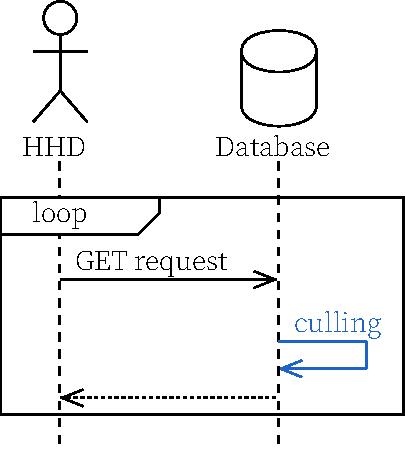
\includegraphics[width=0.38\textwidth]{figures/pdf/first idea.pdf}
	\caption{Sequence diagram - basic concept}
	\label{fig:firstIdea}
\end{figure}


\section{Research questions}\label{sec:researchQuestions}
This thesis proposes the introduction of culling algorithm technology within the context of \ac{ldbim} to address the previously mentioned issue of the scene's size, by culling the scene at its source prior to sending it to the viewer. As culling algorithms have been extensively researched and continue to evolve, as described in section \ref{sec:historyCulling}, the research questions in this thesis concentrate on assessing the feasibility of introducing such algorithms to \ac{ldbim}. It aims to propose a set of possible solutions tailored to this specific problem, while highlighting possibilities for future research and specific use cases.

\subsection[Can \acs{ldbim} be culled?]{To what extent can \acs{ldbim} geometry be culled \\
	to be streamed to lightweight viewers?} \label{subsec:rq1}
In other words, what constitutes the smallest triples (Section \ref{subsec:rdfAndTriples}) or snippets of data required by the viewer and culling algorithms? This question will be addressed by examining possible culling algorithms, their applicability to \ac{ldbim} models, and a hands-on approach to the development of a prototype. This exploration will extend this research question to the implementation of secondary parameters, both from a culling perspective, such as special filters, and from a visual standpoint, such as the visualization of semantics related to each object.

\subsection[Can existing semantics be used?]{Can existing semantics and ontologies be used\\
	to feed possible culling algorithms?}\label{subsec:rq2}
Unlike the computer graphics industry, this interconnected context already includes both explicit and implicit relationships within the graph, the latter being derived through inferencing (Section \ref{subsec:ontologies}). This is similar to the work of \cite{Johansson2009}. In their paper, they utilized the semantics of a \ac{bim} model in \ac{ifc} format to develop culling techniques. However, this thesis will focus on the use of Semantic Web resources. As such, it will examine both \ac{aec}-specific and \ac{aec}-related ontologies, such as those related to \ac{gis}, to determine if they can be employed to feed culling algorithms.

% \section{Research objectives}\label{sec:researchObjectives}
% \subsection[]
% \subsection[Integration in a web viewer]{Integration of the culling algorithms in a modular and extendible web viewer}\label{subsec:ro1}

\chapter{Linked Data}
As mentioned in the \nameref{sec:intro}, the evolution from \ac{bim} to \ac{ldbim} represents an evolution of the data \textbf{management} layer. This layer utilizes \emph{Linked Data} which, as stated by the \ac{w3c}, is a collection of interrelated datasets on the Web, formatted in a standard way that is accessible and manageable by Semantic Web tools. The same applies to the relationships among them.\footcite{w3c} The following collection of Semantic Web technologies explores the required environment to achieve this goal.

\section{\acs{rdf} and triples} \label{subsec:rdfAndTriples}
At the core of the Semantic Web is the \ac{rdf}, a data model for describing resources on the Web. RDF is a graph data model that consists of \textbf{triples}, which are statements about resources. A triple consists of a subject, a predicate, and an object. The subject is the resource that is being described, the predicate is the property of the subject, and the object is the value of the property. Both the predicate and the object can, in turn, become the subjects of other triples. Listing \ref{lst:rdfSample} shows an example of an \ac{rdf} database described in the Turtle format.

\begin{figure}[H]
    \centering
    

\tikzset{every picture/.style={line width=0.75pt}} %set default line width to 0.75pt        

\begin{tikzpicture}[x=0.75pt,y=0.75pt,yscale=-1,xscale=1]
    %uncomment if require: \path (0,300); %set diagram left start at 0, and has height of 300

    %Rounded Rect [id:dp16428191799546488] 
    \draw   (80,68) .. controls (80,63.58) and (83.58,60) .. (88,60) -- (182,60) .. controls (186.42,60) and (190,63.58) .. (190,68) -- (190,92) .. controls (190,96.42) and (186.42,100) .. (182,100) -- (88,100) .. controls (83.58,100) and (80,96.42) .. (80,92) -- cycle ;
    %Rounded Rect [id:dp211253547738401] 
    \draw   (300,68) .. controls (300,63.58) and (303.58,60) .. (308,60) -- (402,60) .. controls (406.42,60) and (410,63.58) .. (410,68) -- (410,92) .. controls (410,96.42) and (406.42,100) .. (402,100) -- (308,100) .. controls (303.58,100) and (300,96.42) .. (300,92) -- cycle ;
    %Straight Lines [id:da3976910390317223] 
    \draw    (190,80) -- (298,80) ;
    \draw [shift={(300,80)}, rotate = 180] [color={rgb, 255:red, 0; green, 0; blue, 0 }  ][line width=0.75]    (10.93,-3.29) .. controls (6.95,-1.4) and (3.31,-0.3) .. (0,0) .. controls (3.31,0.3) and (6.95,1.4) .. (10.93,3.29)   ;

    % Text Node
    \draw (135,80) node   [align=left] {\mintinline[bgcolor=white]{turtle}|flupke:room1|};
    % Text Node
    \draw (355,80) node   [align=left] {\mintinline[bgcolor=white]{turtle}|rdf:type|};
    % Text Node
    \draw (245,66.5) node   [align=left] {\mintinline[bgcolor=white]{turtle}|bot:zone|};
    % Text Node
    \draw (135,113) node  [font=\footnotesize] [align=left] {subject};
    % Text Node
    \draw (355,113) node  [font=\footnotesize] [align=left] {object};
    % Text Node
    \draw (245,92.5) node  [font=\footnotesize] [align=left] {predicate};


\end{tikzpicture}

    \caption{Triple structure}
    \label{fig:triple}
\end{figure}

The basic, yet versatile, structure of a triple is illustrated in Figure \ref{fig:triple}. Both the subject and object are considered as nodes in the data graph, and they are linked by the predicate, which is referred to as an edge. Multiple triples can thus create and link multiple nodes or enrich a connection between two nodes by creating new edges between them. Each element contains a single resource that can be one of the three types: a \acs{uri}, a literal, or a blank node. A \ac{uri} identifies the name and/or location of a resource on the web and, as its name states, is unique and unambiguous, thus enabling queries and reasoning of the same nature. A literal is a value, and a blank node is an anonymous resource, sometimes used as a placeholder when the exact resource is not known or not necessary to specify. Due to their nature, a subject must be either a \ac{uri} or a blank node, a predicate exclusively a \ac{uri}, and the object may be any of the three types. As \ac{uri} descriptions can be very long, a prefix can be used to shorten them. This is illustrated in Listing \ref{lst:rdfSample} with the \mintinline{turtle}|@prefix bot: <https://w3id.org/bot#>|, which declares that \mintinline{turtle}|bot:Zone| refers, in its full length, to the address \mintinline{turtle}|<https://w3id.org/bot#Zone>|.

\begin{listing}[H]
    \inputminted{turtle}{figures/snippets/rdfSample.ttl}
    \vspace{-0.7cm}
    \caption{Example of an \acs{rdf} database in turtle format}
    \label{lst:rdfSample}
\end{listing}

This basic concept can be extrapolated to describe and store any kind of data. The advantage for the \ac{aec} industry would be to allow any stakeholders to describe and enrich the knowledge base of a building.

\section{Ontologies and reasoning}\label{subsec:ontologies}
When looking at Listing \ref{lst:rdfSample}, a distinction can be made between two types of statements: some refer to classes or properties, such as \mintinline{turtle}|bot:Zone| or \mintinline{turtle}|bot:containsElement|, while others refer to instances such as \mintinline{turtle}|flupke:room1|. The former is referred to as the TBox for \enquote{terminology}, and the latter is referred to as the ABox for \enquote{assertions}. The TBox, the ontology layer, is used to describe instances in the ABox and their relationships.

By developing an ontology, the domain of interest and the relationships between the classes and properties can be described. This is achieved by defining the classes and properties of the domain and their relationships. The ontology is then used to reason about the domain, inferring new facts based on the ontology and the existing facts within the domain. This is done by a reasoner, which is software capable of performing the reasoning itself on the ontology and associated data. As mentioned, the reasoner can be used to infer new facts, check if created facts are consistent with the ontology, and check if the ontology itself is consistent.\footcite{w3cInfering} It is often integrated with \ac{rdf} databases, also known as triplestores or graph databases.

Classes, properties, and their relationships can be defined using \ac{rdfs}, which is a vocabulary for describing \ac{rdf} schemas using a basic set of constructs. As an extension of \ac{rdfs}, \ac{owl} is a vocabulary for describing ontologies using a more expressive set of constructs tailored to the needs of ontologies. Both \ac{rdfs} and \ac{owl} are considered to be formal ontologies themselves, as they describe the classes and properties of the domain of \ac{rdf}.

\section{Triplestores and \acs{sparql}}
As briefly discussed in \ref{subsec:ontologies}, triplestores are \ac{rdf} databases that store data in the form of a graph. They are used to store and query Linked Data and are often integrated with a reasoner. The data itself is retrieved and modified using the \ac{sparql}.\footcite{w3cQuery} In contrast to \ac{sql}, \ac{sparql} queries are able to work across multiple triplestores, called \ac{sparql} endpoints. These are known as federated queries, and their results are combined into a single result set. This is useful when the data is distributed across multiple triplestores in a decentralized manner.\footcite{ontotextSpaql} For example, multiple stakeholders participating in a project, each with their own database.

\section{Complexity of the data graph}
The complexity of the data graph is a major concern when working with \ac{ldbim}. This section discusses the origins of the different sources of geometric data that enrich it. Firstly, by looking at the different \ac{lod}'s that can be used to describe a building, which already exists in the \ac{bim} domain. Secondly, by looking at \ac{ldbim} and the exponential growth it imposes on the data graph.

\begin{figure}[H]
    \centering
    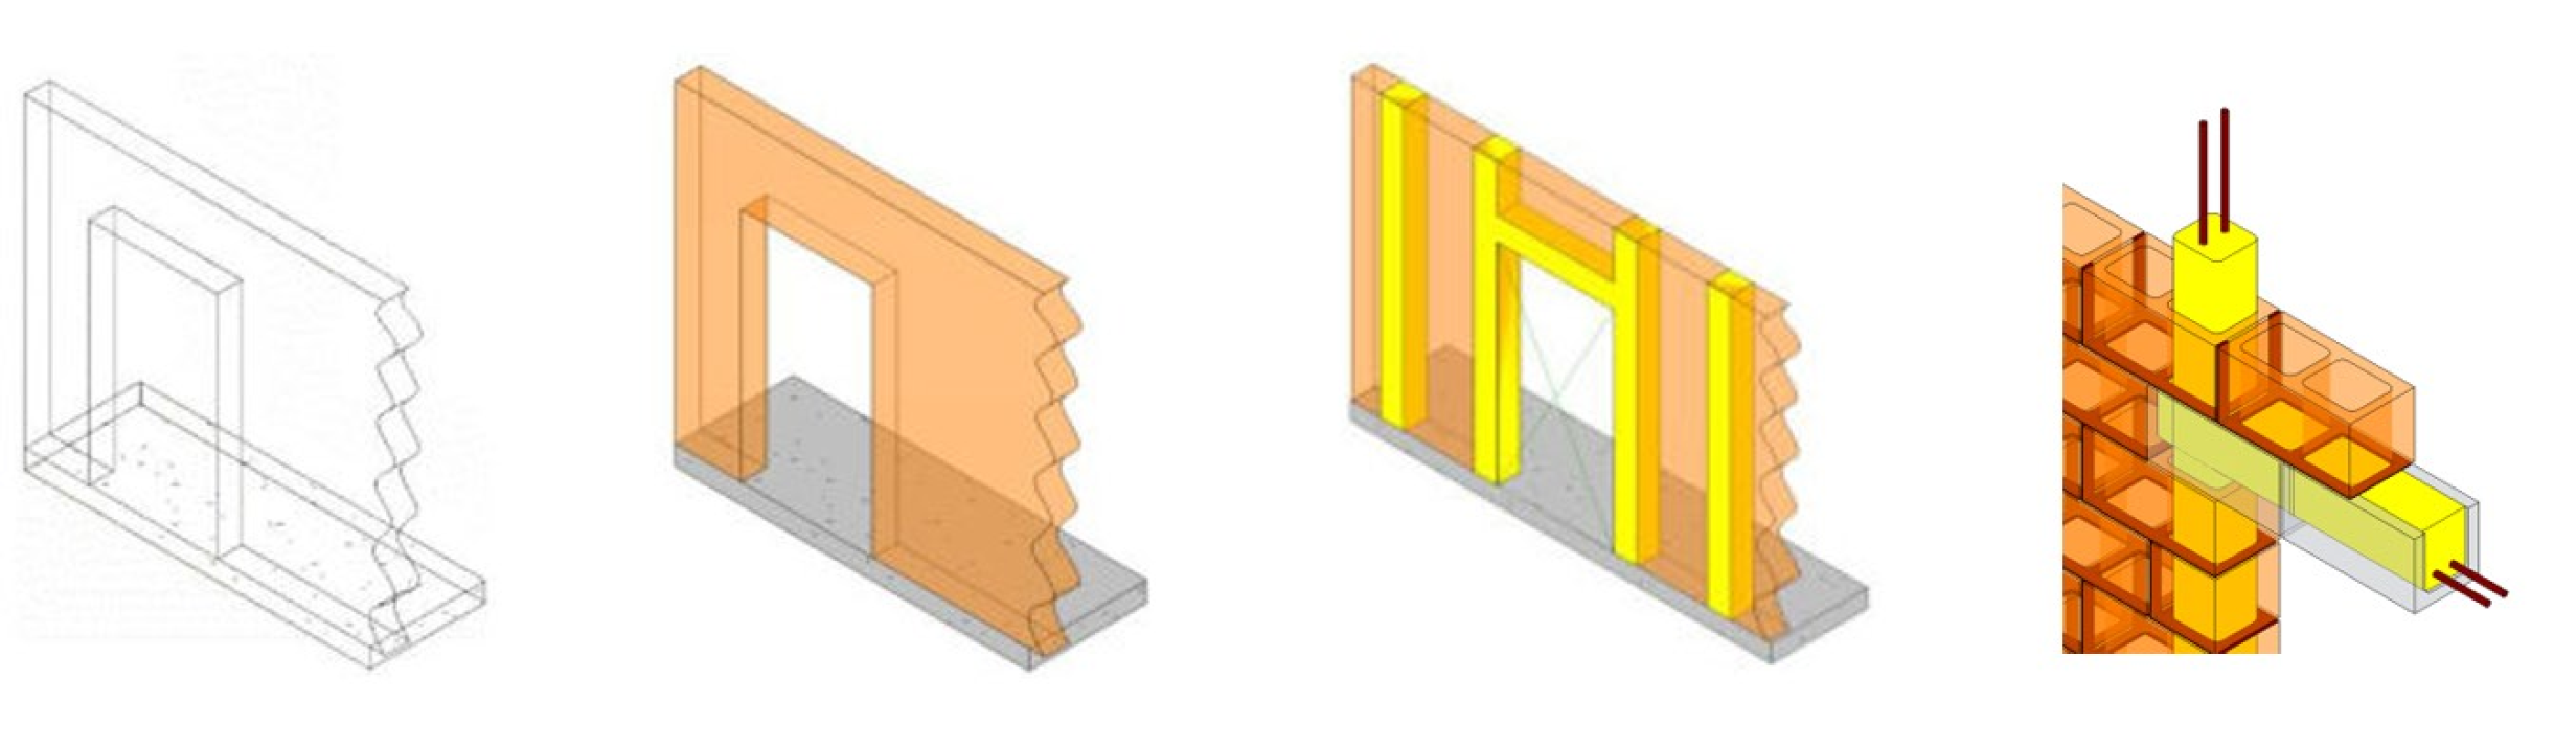
\includegraphics[width=\textwidth]{figures/pdf/LOD.pdf}
    \caption[\acs{lod} evolution]{\acs{lod} evolution\\ from \cite{lod}}
    \label{fig:LOD}
\end{figure}

\subsection{\acs{bim} geometry} \label{subsec:bimGeometry}
The 3D model of a building consists of a multitude of sub-models, describing objects for all the different stakeholders participating in the project. Some describe very large objects, and some very small parts. Both can be defined in their most simple and abstract form or have an intricate and complex geometry. For instance, a door can simply be defined as a box, or up to the level of the screw-thread for the hinge system. The level of abstraction is here described as the \ac{lod}, which is most of the time pre-selected for the needs of a \ac{bim} model, and is applied throughout a single model.

As shown in Figure~\ref{fig:LOD}, a standard BIM workflow goes through multiple phases, each with their associated model and \ac{lod}. This makes it an important concept in the \ac{aec} industry, as it allows for a very efficient workflow. The modeling step is approached from a top-down perspective, starting with rougher geometries describing the broader ideas of a concept model and evolving to a more refined model for the construction documentation phase. As the last and longest-standing model, a higher \ac{lod} can be used to describe subtle changes in the evolution of a building during the operation phase.

\subsection{\acs{ldbim} geometry}
The interconnectivity of semantics can also be applied to geometry descriptions. This could allow the co-existence of multiple \ac{lod}s in a single model database. Besides storing the evolution of a single element's geometry, it enables the linking of the different \ac{lod}s, described in \ref{subsec:bimGeometry}, to each other. Not only that, but extending onto the size of the models described in Table \ref{tab:sizeModels}, already existing \ac{mep}, structural, alongside many other stakeholders' geometry can be added.
\chapter{State of the art} \label{ch:stateOfTheArt}
As mentioned in \cite{Johansson2015}, existing research on the performance of currently used \ac{bim} viewers is quite limited. This state-of-the-art research will, therefore, focus on the overall features of some promising newer viewers and the ontologies/tools that will be used in this thesis.

\section{Existing \acs{bim} viewers and ontologies}
\subsection{Qoniq and \acs{lod} Streaming for \acs{bim}}
Qonic focuses on developing an open platform \ac{bim} viewer. With the use of Unity to enable cross-platform compatibility, they focused on two main aspects: performance and aesthetics. The latter refers to the visual quality of the viewer, offering both a seamless experience for the viewer as well as a pleasant one, with, for example, the implementation of ambient lighting and shadow castings. The first and most researched aspect of their viewer, the performance, is mainly focusing on a \ac{lod} culling algorithm.
\\(T. Strobbe, personal communication, November 25, 2022)

\subsubsection{Qoniq's approach to \acs{lod} streaming}
Their core research is developing a dynamic \ac{lod} streaming model. Starting from the geometry and semantics of an \ac{ifc} file, they compute an \ac{lod} hierarchy tree of the model. Through multiple mesh decimation algorithms, they reduce the number of triangles of each object's mesh, regardless of the semantics associated with that object. On top of that, a filtering algorithm is implemented in the streaming model to filter out objects, regarding their semantics, that are not relevant to the current camera position. In doing so, they both reduce the size of models far from the viewpoint and evaluate the need to show certain objects based on their nature, extracted from semantics in the \ac{ifc} file, and their distance to the camera. The resulting dynamic \ac{lod} streaming model is reevaluated at each camera move in Unity.
\\(T. Strobbe, personal communication, November 25, 2022)

Unity was chosen as it allows for writing once and deploying everywhere. This means that the viewer can be used on any platform, including mobile devices and browsers. The performance results are thus related to the hardware capabilities of each device, with the exception of the browser, where the performance of Unity's WebGL build is limited to a scene size of 2Gb.\footcite{UnityWebGL}

\subsubsection{Advantages and trade-offs}
Being able to run on many platforms, offering a smooth viewer experience and a pleasing aesthetic makes it an ideal candidate for lightweight viewers on the job site. However, the \ac{lod} library has to be computed on every model update. The decimation algorithms are furthermore computational results that are not humanly reviewed. This means that the quality of the resulting meshes is not guaranteed for the lower \ac{lod}s, which are, as illustrated in Figure \ref{fig:LOD}, already modeled in previous design phases. \ac{ldbim} could, by interconnection, recall previous \ac{lod}s in the viewer's scene. Without the need for computational remodeling. Nevertheless, Qonic's approach is already versioning-proof as later \ac{lod}'s may vary from the last design choices. They therefore serve as the goal of this thesis, outside the \ac{ldbim} context.

\subsection{ld-bim.web.app}
\enquote{The purpose of the app is to showcase our LBD toolset and to demonstrate the capabilities of Linked Building Data to newcomers.} \footcite{lbdimApp}

\url{https://ld-bim.web.app/} demonstrates a viewer built around an \ac{rdf} database. It separates the data from an \ac{ifc} file into semantics, stored in the previously mentioned graph, and a glTF model, together with a \ac{json} file containing a reference table. Extra local or remote graphs can be added to the \ac{ui}. As it contains a \ac{sparql} engine to query and visualize, in the form of highlighting, the results of the query in a 3D viewer. The viewer is based on the ifc.js project, which is itself based on the three.js 3D JavaScript library.

\subsection{\acs{aec} related ontologies}
As mentioned in the second research question \ref{subsec:rq2}, this section will discuss \ac{aec}-related technologies that are actively researched by the \ac{lbd-cg}\footcite{lbdOntologies}.

\subsubsection{\acs{bot}}
The \ac{bot} proposes a set of classes and properties, \enquote{which provides a high-level description of the topology of buildings including storeys and spaces, the building elements they may contain, and the 3D mesh geometry of these spaces and elements.} \parencite{Rasmussen2020}, as illustrated in Figure \ref{fig:bot}. This high-level description could be fed to portal-culling algorithms in a situation where the visibility is contained within one \mintinline{turtle}|bot:Space| or \mintinline{turtle}|bot:Storey|, or it could extend the scope to \mintinline{turtle}|bot:adjacentZone|\footcite{GodotPortal}. Additionally, it could play a part in the construction of the \ac{bvh} needed for other occlusion culling algorithms, such as the \ac{chc}++ \parencite{Johansson2015}.

\begin{figure}[H]
    \begin{adjustwidth}{-0.8cm}{-0.8cm}
        \centering
        

\tikzset{every picture/.style={line width=0.75pt}} %set default line width to 0.75pt        

\begin{tikzpicture}[x=0.75pt,y=0.75pt,yscale=-1,xscale=1]
    \ttfamily
%uncomment if require: \path (0,373); %set diagram left start at 0, and has height of 373

%Shape: Parallelogram [id:dp6234888353745478] 
\draw  [fill={rgb, 255:red, 255; green, 253; blue, 237 }  ,fill opacity=0.8 ] (113,261.47) -- (19.33,261.47) -- (53.73,293.8) -- (147.4,293.8) -- cycle ;
%Shape: Parallelogram [id:dp5369889401184471] 
\draw  [fill={rgb, 255:red, 255; green, 253; blue, 237 }  ,fill opacity=1 ] (482.33,150) -- (182.41,150) -- (280.07,250) -- (580,250) -- cycle ;
%Shape: Cube [id:dp8255469967169493] 
\draw  [fill={rgb, 255:red, 243; green, 255; blue, 228 }  ,fill opacity=0.8 ] (530,173.85) -- (475.75,119.6) -- (272.41,119.6) -- (272.41,165.35) -- (326.66,219.6) -- (530,219.6) -- cycle ; \draw   (272.41,119.6) -- (326.66,173.85) -- (530,173.85) ; \draw   (326.66,173.85) -- (326.66,219.6) ;
%Shape: Cube [id:dp7451550676115966] 
\draw  [fill={rgb, 255:red, 254; green, 235; blue, 202 }  ,fill opacity=0.8 ] (530,134.25) -- (475.75,80) -- (272.41,80) -- (272.41,105.75) -- (326.66,160) -- (530,160) -- cycle ; \draw   (272.41,80) -- (326.66,134.25) -- (530,134.25) ; \draw   (326.66,134.25) -- (326.66,160) ;
%Shape: Cube [id:dp7376474366082748] 
\draw  [fill={rgb, 255:red, 220; green, 236; blue, 254 }  ,fill opacity=0.8 ] (457.41,76.33) -- (421.07,40) -- (272.41,40) -- (272.41,63.67) -- (308.74,100) -- (457.41,100) -- cycle ; \draw   (272.41,40) -- (308.74,76.33) -- (457.41,76.33) ; \draw   (308.74,76.33) -- (308.74,100) ;
%Shape: Cube [id:dp6037678452495017] 
\draw  [fill={rgb, 255:red, 254; green, 220; blue, 220 }  ,fill opacity=0.8 ][line width=0.75]  (498.07,46.33) -- (461.74,10) -- (312.41,10) -- (312.41,33.67) -- (348.74,70) -- (498.07,70) -- cycle ; \draw  [line width=0.75]  (312.41,10) -- (348.74,46.33) -- (498.07,46.33) ; \draw  [line width=0.75]  (348.74,46.33) -- (348.74,70) ;
%Curve Lines [id:da34503747339894364] 
\draw  [dash pattern={on 0.84pt off 2.51pt}]  (617.81,114.6) .. controls (634.52,117.78) and (665.49,69.49) .. (494.4,64.67) ;
\draw [shift={(491.81,64.6)}, rotate = 1.45] [fill={rgb, 255:red, 0; green, 0; blue, 0 }  ][line width=0.08]  [draw opacity=0] (3.57,-1.72) -- (0,0) -- (3.57,1.72) -- cycle    ;
%Curve Lines [id:da8352390399084118] 
\draw  [dash pattern={on 0.84pt off 2.51pt}]  (617.81,107.8) .. controls (628.61,105.4) and (659.41,85.8) .. (449.81,94.6) ;
\draw [shift={(449.81,94.6)}, rotate = 357.6] [fill={rgb, 255:red, 0; green, 0; blue, 0 }  ][line width=0.08]  [draw opacity=0] (3.57,-1.72) -- (0,0) -- (3.57,1.72) -- cycle    ;
%Curve Lines [id:da4764695659197302] 
\draw  [dash pattern={on 0.84pt off 2.51pt}]  (637.81,186.6) .. controls (660.61,192.6) and (716.61,57) .. (491.81,58.6) ;
\draw [shift={(491.81,58.6)}, rotate = 359.59] [fill={rgb, 255:red, 0; green, 0; blue, 0 }  ][line width=0.08]  [draw opacity=0] (3.57,-1.72) -- (0,0) -- (3.57,1.72) -- cycle    ;
%Curve Lines [id:da6997716856913325] 
\draw  [dash pattern={on 0.84pt off 2.51pt}]  (637.81,181.4) .. controls (653.41,183.8) and (664.21,139.4) .. (649.81,116.2) .. controls (635.48,93.12) and (638.97,82.7) .. (452.63,88.51) ;
\draw [shift={(449.81,88.6)}, rotate = 358.18] [fill={rgb, 255:red, 0; green, 0; blue, 0 }  ][line width=0.08]  [draw opacity=0] (3.57,-1.72) -- (0,0) -- (3.57,1.72) -- cycle    ;
%Curve Lines [id:da2611543315656344] 
\draw  [dash pattern={on 0.84pt off 2.51pt}]  (637.21,176.6) .. controls (656.91,177.4) and (651.86,138.99) .. (477.25,150.82) ;
\draw [shift={(474.61,151)}, rotate = 356] [fill={rgb, 255:red, 0; green, 0; blue, 0 }  ][line width=0.08]  [draw opacity=0] (3.57,-1.72) -- (0,0) -- (3.57,1.72) -- cycle    ;
%Curve Lines [id:da3444743375210677] 
\draw  [dash pattern={on 0.84pt off 2.51pt}]  (571.41,279.4) .. controls (618.61,279.4) and (830.21,63.4) .. (491.41,52.2) ;
\draw [shift={(491.41,52.2)}, rotate = 1.89] [fill={rgb, 255:red, 0; green, 0; blue, 0 }  ][line width=0.08]  [draw opacity=0] (3.57,-1.72) -- (0,0) -- (3.57,1.72) -- cycle    ;
%Curve Lines [id:da00012227444950441146] 
\draw  [dash pattern={on 0.84pt off 2.51pt}]  (571.81,269.8) .. controls (588.81,272.6) and (679.01,195) .. (653.01,168.6) .. controls (627.27,142.46) and (556.83,139.46) .. (477.03,144.45) ;
\draw [shift={(474.61,144.6)}, rotate = 356.32] [fill={rgb, 255:red, 0; green, 0; blue, 0 }  ][line width=0.08]  [draw opacity=0] (3.57,-1.72) -- (0,0) -- (3.57,1.72) -- cycle    ;
%Curve Lines [id:da2737876317435528] 
\draw  [dash pattern={on 0.84pt off 2.51pt}]  (571.81,265.8) .. controls (591.51,266.6) and (641.3,212.35) .. (477.89,209.44) ;
\draw [shift={(475.41,209.4)}, rotate = 0.83] [fill={rgb, 255:red, 0; green, 0; blue, 0 }  ][line width=0.08]  [draw opacity=0] (3.57,-1.72) -- (0,0) -- (3.57,1.72) -- cycle    ;
%Curve Lines [id:da48651030268326223] 
\draw  [dash pattern={on 0.84pt off 2.51pt}]  (571.81,275.4) .. controls (591.47,275.4) and (678.21,205.8) .. (675.41,141) .. controls (672.62,76.52) and (587.07,81.75) .. (451.85,82.19) ;
\draw [shift={(449.81,82.2)}, rotate = 359.83] [fill={rgb, 255:red, 0; green, 0; blue, 0 }  ][line width=0.08]  [draw opacity=0] (3.57,-1.72) -- (0,0) -- (3.57,1.72) -- cycle    ;
%Straight Lines [id:da018272292431112502] 
\draw  [dash pattern={on 4.5pt off 4.5pt}]  (152.41,20) -- (312.41,20) ;
%Straight Lines [id:da7335835552603491] 
\draw  [dash pattern={on 4.5pt off 4.5pt}]  (152.41,50) -- (272.41,50) ;
%Straight Lines [id:da8480379890588858] 
\draw  [dash pattern={on 4.5pt off 4.5pt}]  (152.41,90) -- (272.41,90) ;
%Straight Lines [id:da5645617535440737] 
\draw  [dash pattern={on 4.5pt off 4.5pt}]  (152.41,130) -- (272.41,130) ;
%Straight Lines [id:da7578549164754749] 
\draw  [dash pattern={on 4.5pt off 4.5pt}]  (152.41,180) -- (212.41,180) ;
%Straight Lines [id:da4046157540132602] 
\draw    (35,10) -- (35,190) ;
%Straight Lines [id:da9585577369264056] 
\draw    (35,10) -- (45,10) ;
%Straight Lines [id:da8679205527736427] 
\draw    (35,190) -- (45,190) ;
%Straight Lines [id:da4346199951984231] 
\draw    (265.4,219) -- (328.83,210.59) ;
\draw [shift={(331.8,210.2)}, rotate = 172.45] [fill={rgb, 255:red, 0; green, 0; blue, 0 }  ][line width=0.08]  [draw opacity=0] (3.57,-1.72) -- (0,0) -- (3.57,1.72) -- cycle    ;
%Straight Lines [id:da9955272147380352] 
\draw    (275.7,149.72) -- (330,149.99) ;
\draw [shift={(333,150)}, rotate = 180.28] [fill={rgb, 255:red, 0; green, 0; blue, 0 }  ][line width=0.08]  [draw opacity=0] (3.57,-1.72) -- (0,0) -- (3.57,1.72) -- cycle    ;
%Straight Lines [id:da5290759611186164] 
\draw    (268.7,101.72) -- (312.47,92.42) ;
\draw [shift={(315.4,91.8)}, rotate = 168.01] [fill={rgb, 255:red, 0; green, 0; blue, 0 }  ][line width=0.08]  [draw opacity=0] (3.57,-1.72) -- (0,0) -- (3.57,1.72) -- cycle    ;
%Straight Lines [id:da2082247372760495] 
\draw    (307.8,32.6) -- (351.1,53.69) ;
\draw [shift={(353.8,55)}, rotate = 205.96] [fill={rgb, 255:red, 0; green, 0; blue, 0 }  ][line width=0.08]  [draw opacity=0] (3.57,-1.72) -- (0,0) -- (3.57,1.72) -- cycle    ;
%Shape: Cube [id:dp41271376617212563] 
\draw  [fill={rgb, 255:red, 243; green, 255; blue, 228 }  ,fill opacity=0.8 ] (120,251) -- (105,236) -- (40,236) -- (40,271) -- (55,286) -- (120,286) -- cycle ; \draw   (40,236) -- (55,251) -- (120,251) ; \draw   (55,251) -- (55,286) ;
%Shape: Cube [id:dp24709864473657217] 
\draw  [fill={rgb, 255:red, 254; green, 235; blue, 202 }  ,fill opacity=0.8 ] (120,251.17) -- (104.83,236) -- (40,236) -- (40,250.83) -- (55.17,266) -- (120,266) -- cycle ; \draw   (40,236) -- (55.17,251.17) -- (120,251.17) ; \draw   (55.17,251.17) -- (55.17,266) ;
%Shape: Cube [id:dp7279118293384432] 
\draw  [fill={rgb, 255:red, 220; green, 236; blue, 254 }  ,fill opacity=0.8 ] (90,243.83) -- (82.17,236) -- (40,236) -- (40,250.67) -- (47.83,258.5) -- (90,258.5) -- cycle ; \draw   (40,236) -- (47.83,243.83) -- (90,243.83) ; \draw   (47.83,243.83) -- (47.83,258.5) ;
%Shape: Cube [id:dp46117172286245767] 
\draw  [fill={rgb, 255:red, 254; green, 220; blue, 220 }  ,fill opacity=0.8 ] (97.83,251.17) -- (90.5,243.83) -- (47.83,243.83) -- (47.83,258.5) -- (55.17,265.83) -- (97.83,265.83) -- cycle ; \draw   (47.83,243.83) -- (55.17,251.17) -- (97.83,251.17) ; \draw   (55.17,251.17) -- (55.17,265.83) ;
%Curve Lines [id:da718845720785724] 
\draw    (282.08,336.27) .. controls (289.17,314.99) and (337.4,313.12) .. (376.69,312.69) ;
\draw [shift={(378.48,312.67)}, rotate = 179.42] [color={rgb, 255:red, 0; green, 0; blue, 0 }  ][line width=0.75]    (10.93,-3.29) .. controls (6.95,-1.4) and (3.31,-0.3) .. (0,0) .. controls (3.31,0.3) and (6.95,1.4) .. (10.93,3.29)   ;
%Curve Lines [id:da5183556614244442] 
\draw  [dash pattern={on 0.84pt off 2.51pt}]  (480.48,334.67) .. controls (487.57,313.39) and (535.8,311.52) .. (575.09,311.09) ;
\draw [shift={(576.88,311.07)}, rotate = 179.42] [color={rgb, 255:red, 0; green, 0; blue, 0 }  ][line width=0.75]    (10.93,-3.29) .. controls (6.95,-1.4) and (3.31,-0.3) .. (0,0) .. controls (3.31,0.3) and (6.95,1.4) .. (10.93,3.29)   ;

% Text Node
\draw (276.69,228) node [anchor=north west][inner sep=0.75pt]  [xslant=-0.93] [align=left] {flupke:siteX};
% Text Node
\draw (332.74,199.33) node [anchor=north west][inner sep=0.75pt]  [font=\small] [align=left] {flupke:buildingA \ \ \ \ \ \ \ \ \ \ };
% Text Node
\draw (333.41,142) node [anchor=north west][inner sep=0.75pt]  [font=\small] [align=left] {flupke:storey01 \ \ \ \ \ \ \ \ \ \ };
% Text Node
\draw (355.41,53) node [anchor=north west][inner sep=0.75pt]  [font=\footnotesize] [align=left] {flupke:spaceA12 \ \ \ \ \ \ \ \ \ \ };
% Text Node
\draw  [fill={rgb, 255:red, 255; green, 255; blue, 255 }  ,fill opacity=1 ]  (480.41,101) -- (617.41,101) -- (617.41,122) -- (480.41,122) -- cycle  ;
\draw (483.41,105) node [anchor=north west][inner sep=0.75pt]  [font=\footnotesize] [align=left] {bot:containsZone \ \ \ \ \ \ \ \ \ \ };
% Text Node
\draw  [fill={rgb, 255:red, 255; green, 255; blue, 255 }  ,fill opacity=1 ]  (500.41,171) -- (636.41,171) -- (636.41,191) -- (500.41,191) -- cycle  ;
\draw (503.41,175) node [anchor=north west][inner sep=0.75pt]  [font=\footnotesize] [align=left] {bot:containsZone \ \ \ \ \ \ \ \ \ \ };
% Text Node
\draw  [fill={rgb, 255:red, 255; green, 255; blue, 255 }  ,fill opacity=1 ]  (434.41,261) -- (570.41,261) -- (570.41,281) -- (434.41,281) -- cycle  ;
\draw (437.41,265) node [anchor=north west][inner sep=0.75pt]  [font=\footnotesize] [align=left] {bot:containsZone \ \ \ \ \ \ \ \ \ \ };
% Text Node
\draw (315.41,83) node [anchor=north west][inner sep=0.75pt]  [font=\footnotesize] [align=left] {flupke:spaceA12 \ \ \ \ \ \ \ \ \ \ };
% Text Node
\draw (145.41,20.5) node [anchor=east] [inner sep=0.75pt]  [font=\small] [align=left] {bot:Space};
% Text Node
\draw (145.41,49.5) node [anchor=east] [inner sep=0.75pt]  [font=\small] [align=left] {bot:Space};
% Text Node
\draw (145.41,89.5) node [anchor=east] [inner sep=0.75pt]  [font=\small] [align=left] {bot:Storey};
% Text Node
\draw (145.41,129.5) node [anchor=east] [inner sep=0.75pt]  [font=\small] [align=left] {bot:Building};
% Text Node
\draw (145.41,179.5) node [anchor=east] [inner sep=0.75pt]  [font=\small] [align=left] {bot:Site};
% Text Node
\draw (20.5,100.5) node  [font=\normalsize,rotate=-270] [align=left] {bot:Zone};
% Text Node
\draw  [fill={rgb, 255:red, 255; green, 255; blue, 255 }  ,fill opacity=1 ]  (138,208) -- (268,208) -- (268,228) -- (138,228) -- cycle  ;
\draw (141,212) node [anchor=north west][inner sep=0.75pt]  [font=\footnotesize] [align=left] {bot:hasBuilding \ \ \ \ \ \ \ \ \ \ \ };
% Text Node
\draw  [fill={rgb, 255:red, 255; green, 255; blue, 255 }  ,fill opacity=1 ]  (168,141) -- (280,141) -- (280,161) -- (168,161) -- cycle  ;
\draw (171,145) node [anchor=north west][inner sep=0.75pt]  [font=\footnotesize] [align=left] {bot:hasStorey \ \ \ \ \ \ \ \ };
% Text Node
\draw  [fill={rgb, 255:red, 255; green, 255; blue, 255 }  ,fill opacity=1 ]  (171,25) -- (308,25) -- (308,46) -- (171,46) -- cycle  ;
\draw (174,29) node [anchor=north west][inner sep=0.75pt]  [font=\footnotesize] [align=left] {bot:adjacentZone \ \ \ \ \ \ \ \ \ \ };
% Text Node
\draw  [fill={rgb, 255:red, 255; green, 255; blue, 255 }  ,fill opacity=1 ]  (171,95) -- (275,95) -- (275,115) -- (171,115) -- cycle  ;
\draw (174,99) node [anchor=north west][inner sep=0.75pt]  [font=\footnotesize] [align=left] {bot:hasSpace \ \ \ \ \ \ };
% Text Node
\draw  [fill={rgb, 255:red, 255; green, 255; blue, 255 }  ,fill opacity=1 ]  (110.74,314.83) -- (262.74,314.83) -- (262.74,334.83) -- (110.74,334.83) -- cycle  ;
\draw (113.74,318.83) node [anchor=north west][inner sep=0.75pt]  [font=\footnotesize] [align=left] {owl:ObjectProperty \ \ \ \ \ \ \ \ \ \ \ \ };
% Text Node
\draw (301.04,322.88) node [anchor=north west][inner sep=0.75pt]  [font=\small] [align=left] {explicitly stated};
% Text Node
\draw (498.64,322.88) node [anchor=north west][inner sep=0.75pt]  [font=\small] [align=left] {inferred};
% Connection
\draw  [dash pattern={on 0.84pt off 2.51pt}]  (353.59,249) .. controls (378.56,263.15) and (405.5,269.14) .. (434.41,266.98) ;
% Connection
\draw  [dash pattern={on 0.84pt off 2.51pt}]  (414.39,195.33) .. controls (417.83,184.2) and (459.52,178.83) .. (500.41,180.89) ;
% Connection
\draw  [dash pattern={on 0.84pt off 2.51pt}]  (411,138) .. controls (426.16,116.24) and (468.16,106.77) .. (480.41,111.68) ;
% Connection
\draw    (271.82,235.25) .. controls (248.39,234.24) and (195.05,236.49) .. (207.18,228) ;
% Connection
\draw    (329.74,201.67) .. controls (289.49,202.06) and (252.87,191.28) .. (231.88,161) ;
% Connection
\draw    (330.41,141.89) .. controls (315.58,140.78) and (232.01,133.24) .. (230.12,115) ;
% Connection
\draw    (312.41,84.59) .. controls (286.33,87.84) and (248.33,73.82) .. (242.66,45) ;

\end{tikzpicture}

        \vspace{-0.3cm}
        \caption[Illustration of the \acs{bot} ontology]{Illustration of the \acs{bot} ontology, based on \cite{Rasmussen2020}.}
        \label{fig:bot}
    \end{adjustwidth}
\end{figure}

\subsubsection{\acs{fog} and \acs{omg}} \label{sec:fog}
With the help of \ac{fog} and \ac{omg}, geometry descriptions can be linked in the data graph. The innovation lies in the choice to store it either inside or outside the graph, by means of one triple referring to a literal or an \ac{uri}. Listing \ref{lst:rdfSample} showcases multiple examples of objects assigned with a geometry description using an \ac{uri}\parencite{Bonduel2019}.

\begin{listing}[H]
    \begin{minted}{turtle}
flupke:coneOBJ_geometry-1 fog:asObj_v3.0-obj "https://..."^^xsd:anyURI .
    \end{minted}
    \vspace{-0.7cm}
    \caption{Example of \acs{fog} usage}
    \label{lst:fogSample}
\end{listing}

Listing \ref{lst:fogSample} describes a subject of datatype \mintinline{turtle}|xsd:anyURI| from the \ac{xsd}\footcites{xsd}. The versatile approach of \cite{Bonduel2019} also proposes the following datatypes: \mintinline{turtle}|xsd:string| for \ac{ascii}-based geometry descriptions or \mintinline{turtle}|xsd:base64Binary| for binary geometry descriptions.

The format of the geometry is assigned directly by the predicate in Listing \ref{lst:fogSample}, which is \mintinline{turtle}|fog:asObj_v3.0-obj|. This further infers the statements in Listing \ref{lst:fogInference}.\footcite{fog}

\begin{listing}[H]
    \begin{minted}{turtle}
flupke:coneOBJ_geometry-1 fog:asObj "https://..."^^xsd:anyURI ;
    ex:LOD "100"^^xsd:integer .
    \end{minted}
    \vspace{-0.7cm}
    \caption{\acs{fog} inference examples}
    \label{lst:fogInference}
\end{listing}

The possibility of introducing an external geometry location adds a new participant to Figure \ref{fig:firstIdea}, the external database, from which some files are expected to be fetched. This is illustrated in Figure \ref{fig:3participants}.

\begin{figure}[H]
    \centering
    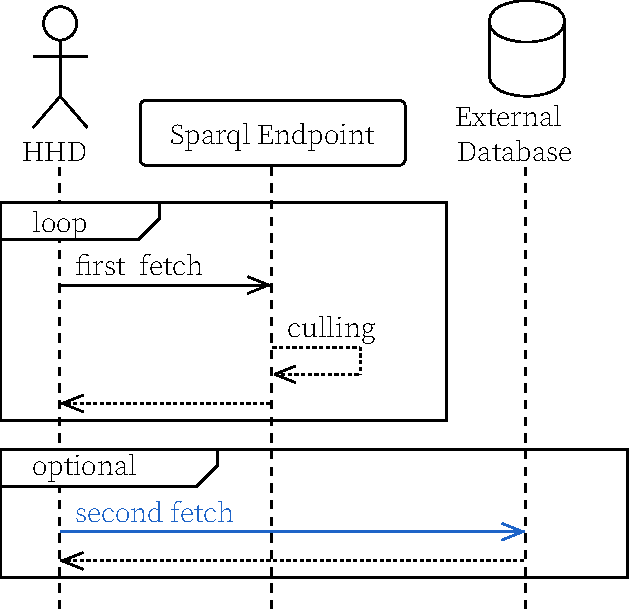
\includegraphics[width=0.6\textwidth]{figures/pdf/3participants.pdf}
    \caption{Sequence diagram with external database - concept}
    \label{fig:3participants}
\end{figure}

\cite{Bonduel2019} refers to the proposal of the \ac{lbd-cg} stated in \cite{holten2018opm} to write Linked Data patterns on three possible levels, \enquote{each having a different degree of complexity}. The first and second levels are illustrated in Figure \ref{fig:fogGom}. Level 2 allows assigning multiple geometry descriptions to a single object, each with, for example, a different \ac{lod}.

\begin{figure}[H]
    \begin{adjustwidth}{-0.8cm}{-0.8cm}
        \centering
        \ttfamily
        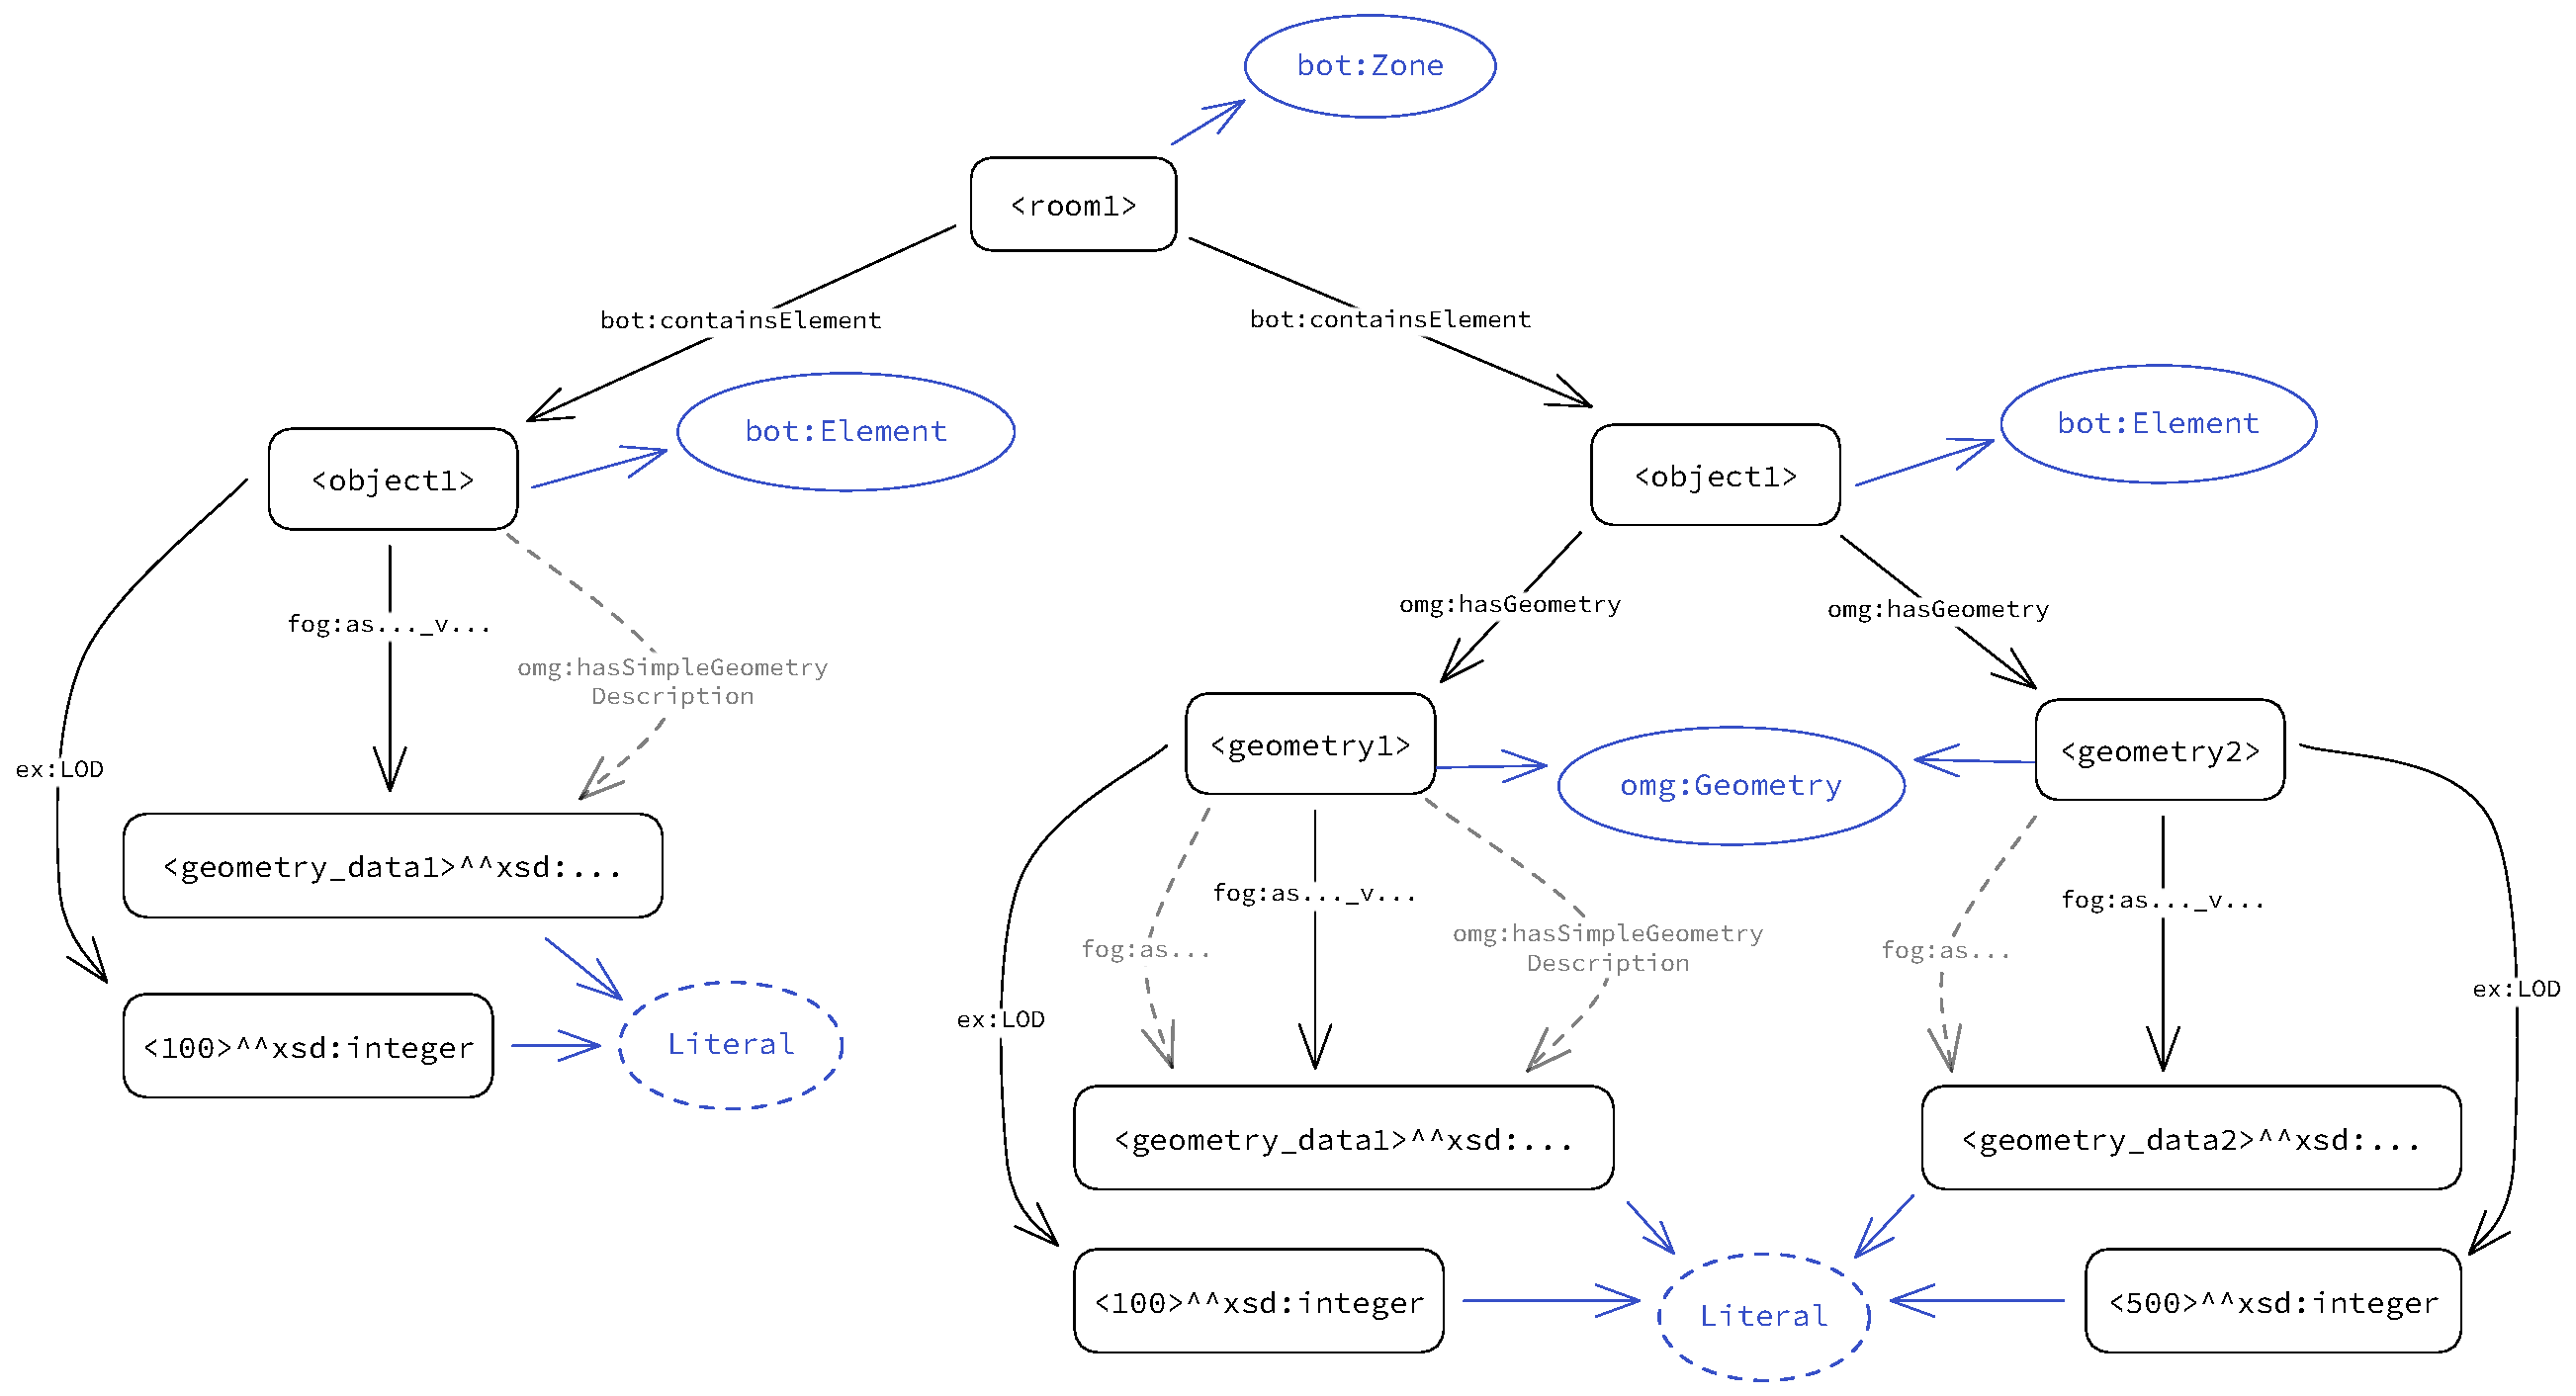
\includegraphics[width=1.1\textwidth]{figures/pdf/fog-omg.pdf}
        \caption[Illustration of the \acs{fog} and \acs{omg} ontologies]{Illustration of Level 1 (left) and Level 2 (right) of the \acs{fog} and \acs{omg} ontologies, based on \cite{Bonduel2019}.}
        \label{fig:fogGom}
    \end{adjustwidth}
\end{figure}

\subsection{\acs{gis} related ontologies}
The technological field of study, \acf{gis}, is closely related to the \ac{bim} domain. The central standards organization, \ac{ogc}, which actively maintains the \ac{gis} standards, is also prominent in the Semantic Web scene. They recognize widely adopted standards such as GeoSPARQL.\footcite{OGC2023SW}

\subsubsection{GeoSPARQL}
\enquote{The OGC GeoSPARQL standard supports representing and querying geospatial data on the Semantic Web. GeoSPARQL defines a vocabulary for representing geospatial data in RDF, and it defines an extension to the SPARQL query language for processing geospatial data. In addition, GeoSPARQL is designed to accommodate systems based on qualitative spatial reasoning and systems based on quantitative spatial computations.} \footcite{OGC2023}

As multiple triplestores and \ac{sparql} endpoints support the GeoSPARQL extension, it is a viable candidate for spatial and \ac{lod} culling algorithms. Such algorithms require spatial data, such as the distance from the viewpoint to the object. Spatial query functions proposed in this extension are needed for this purpose. The functions can compute on nodes of geospatial geometry as if they are expressed using \ac{wkt} or the \ac{gml}. These expressions can be assigned by using the predicates \mintinline{turtle}|geo:asWKT| or \mintinline{turtle}|geo:asGML|. However, GeoSPARQL comes with some limitations that are less prevalent in the \ac{gis} domain, which mostly requires 2D data \parencite{perry2012ogc}, in contrast to \ac{bim} where 3D distance functions would be needed. Despite such limitations, GeoSPARQL remains a viable solution for spatial querying, and workarounds could be employed to address them.

\section{On the market viewers comparison}
\cite{Johansson2015} mentioned in their paper the lack of research about objective \ac{bim} viewers comparison and made one as a result. The size of the model they tested can be found in Table \ref{tab:sizeModels}. They evaluted the following viewers:
\begin{itemize}
    \item DDS CAD Viewer
    \item Tekla BIMsight
    \item Autodesk Navisworks
    \item Solibri Model Viewer
\end{itemize}

\subsection{General Features}
Their study had two main goals. Firstly, evaluating existing viewers and their capabilities, they identified the acceleration techniques used, which are presented in Table \ref{tab:accelerationTechniques}.

\begin{table}[H]
    \centering
    \begin{tabular}{ll}
        \toprule
        \acs{bim} viewer & Acceleration technique                                                                                                                  \\ \midrule
        Solibri 9.0      & \acs{vfc} | \acs{dc} (optional) | \acs{hagi} (optional)                                                                                 \\
        Naviswork 2015   & \begin{tabular}[c]{@{}l@{}}\acs{vfc} | \acs{dc} (optional) | \acs{cpu} \acs{oc} (optional)\\ \acs{gpu} \acs{oc} (optional)\end{tabular} \\
        BIMSight 1.9.1   & \acs{vfc}                                                                                                                               \\
        DDS 8.0          & \acs{vfc} | \acs{dc} (optional)                                                                                                         \\
        DDS 10.0         & \acs{vfc} | \acs{dc}                                                                                                                    \\ \bottomrule
    \end{tabular}
    \caption[Acceleration techniques used by tested viewers]{Acceleration techniques used by tested viewers from \cite{Johansson2015}. {\footnotesize (\acf{vfc}, \acf{dc}, \acf{hagi}, \acf{cpu}, \acf{oc})}}
    \label{tab:accelerationTechniques}
\end{table}

Secondly, they implemented modern culling algorithms and strategies such as \ac{chc}++. The worst-case scenarios are shown in Figure \ref{fig:performanceJohansson} against the Solibri viewer. The results are quite promising, but as concluded by the authors, the gains are limited to the capacities of the \ac{gpu}, \ac{vram}, and \ac{ram}, as discussed in \ref{sec:researchQuestions}.

\begin{figure}[H]
    \centering
    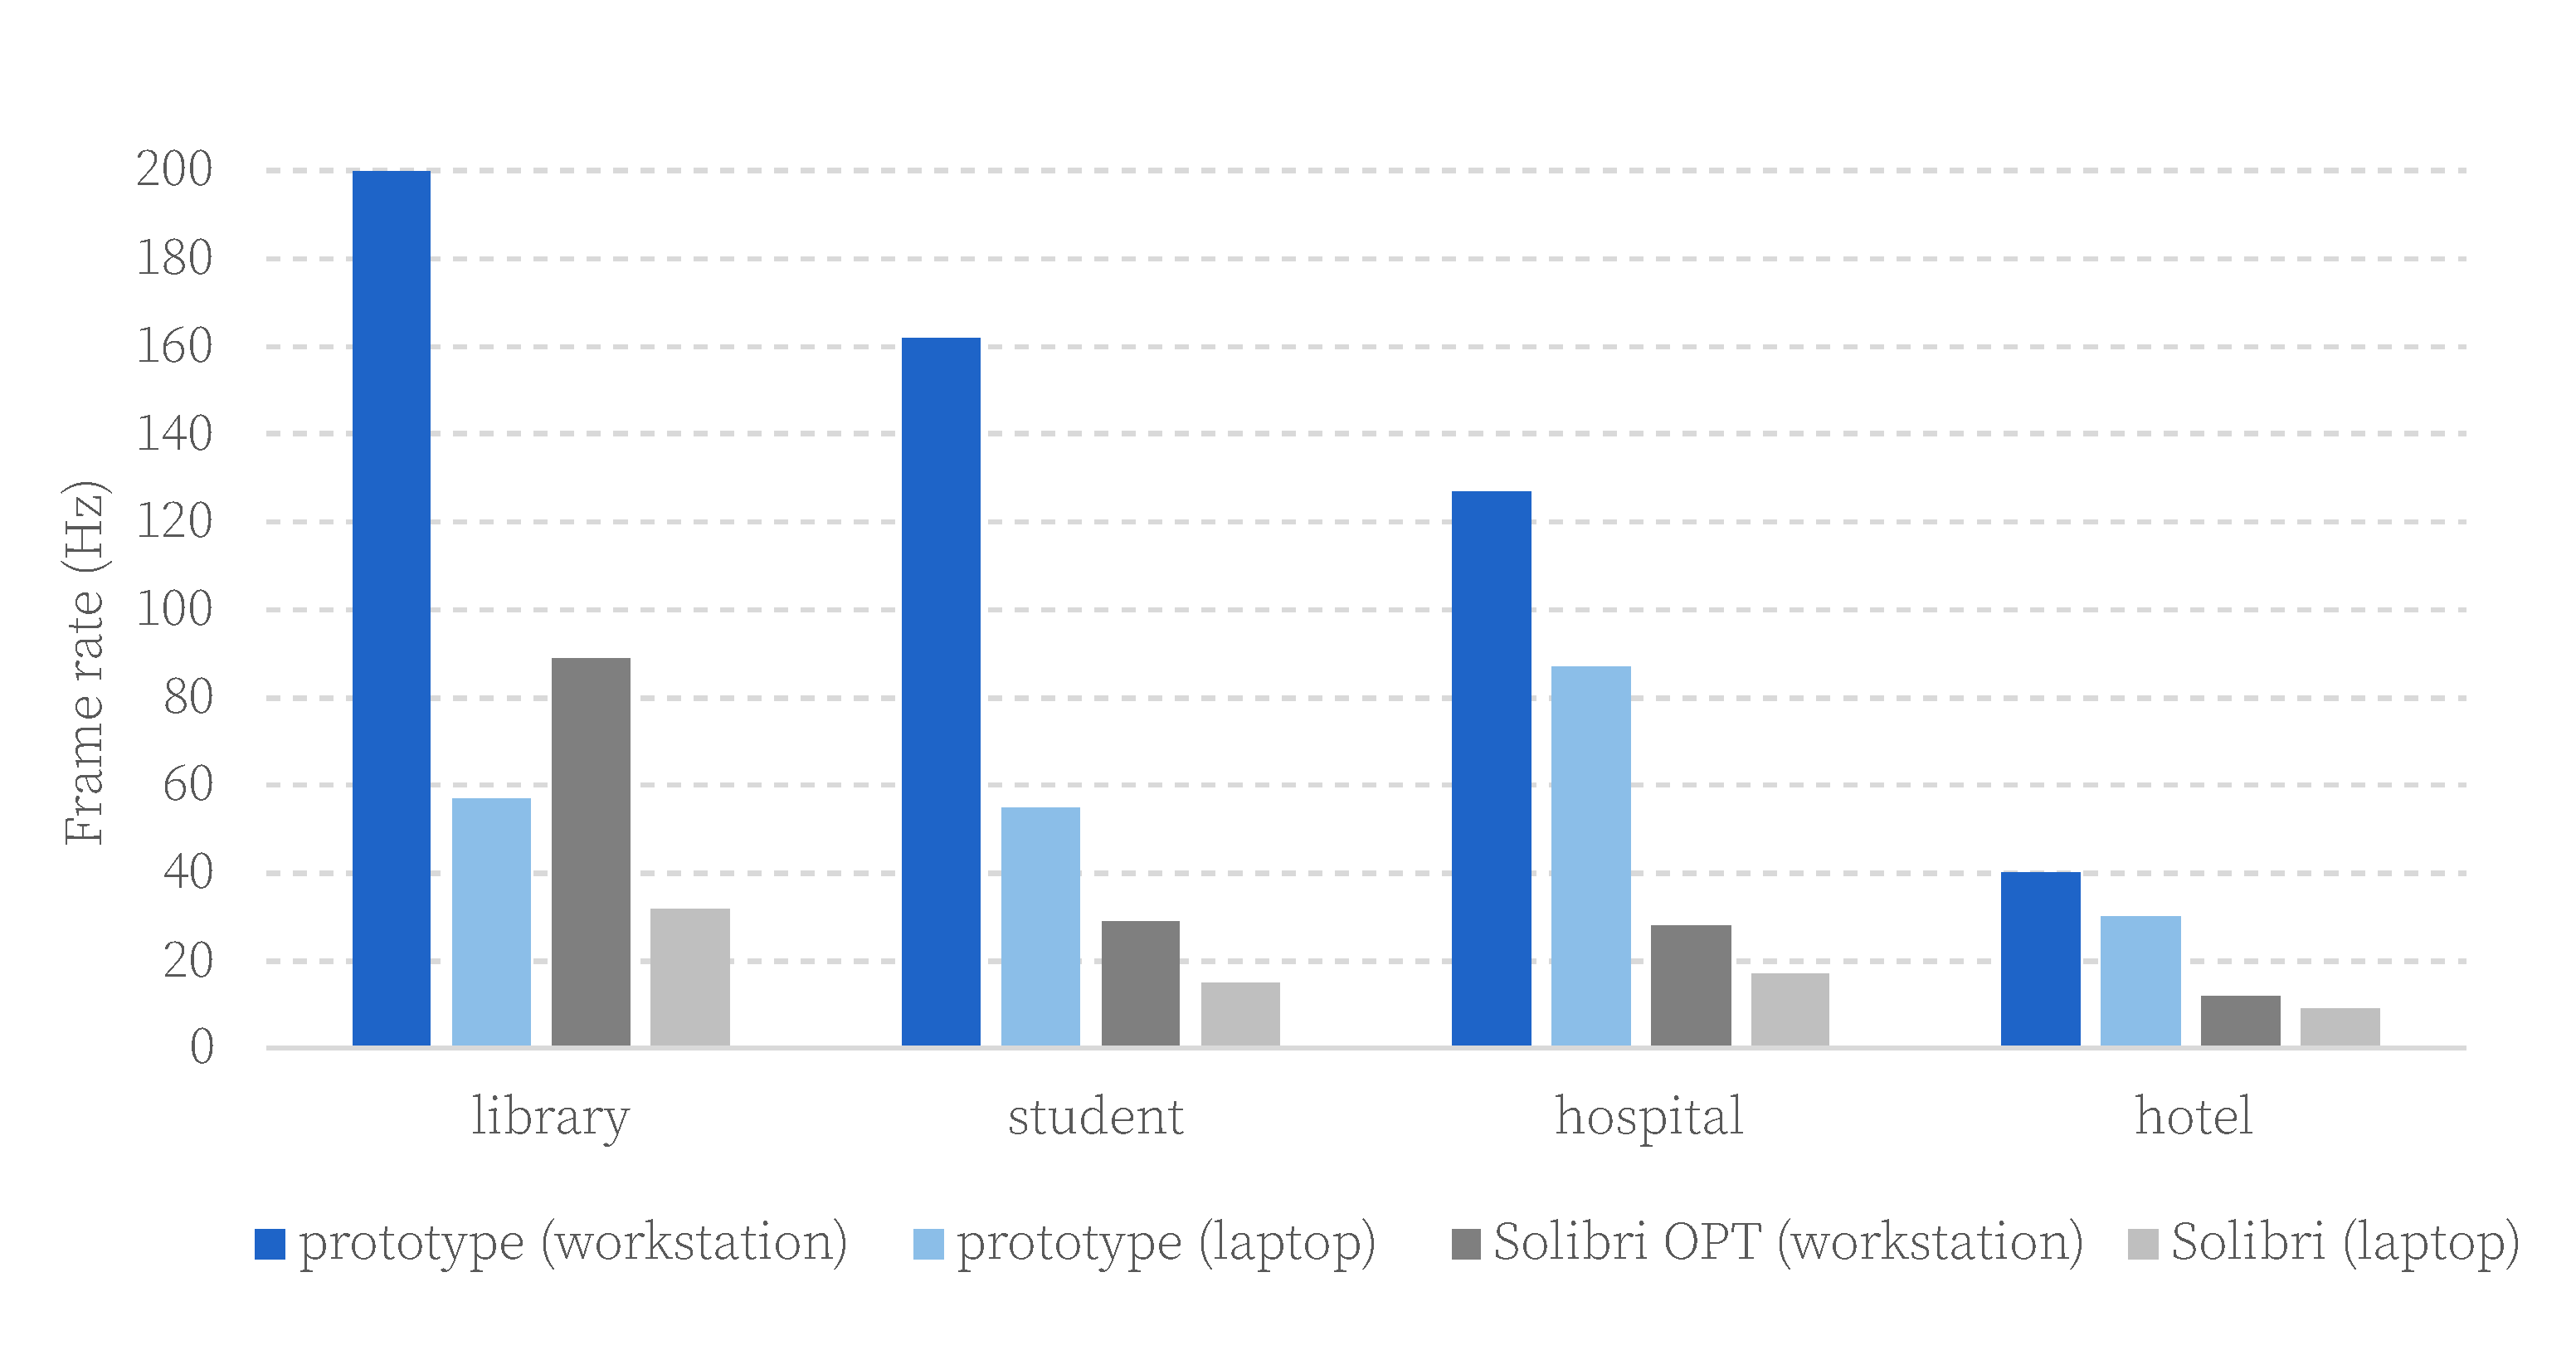
\includegraphics[width=\textwidth]{figures/pdf/JohanssonPerformances.pdf}
    \caption[Performance viewers]{Comparison in rendering performance.\\ from \cite{Johansson2015}}
    \label{fig:performanceJohansson}
\end{figure}

\section{Culling algorithms}\label{sec:historyCulling}
\cite{Johansson2015} presented in their paper a new \ac{bim} viewer equipped with the powerful \ac{chc}++. This is a third-generation occlusion culling algorithm developed by \cite{Mattausch2008}, the first being the \ac{chc} \parencite{Bittner2004}, followed by the \ac{nohc} \parencite{Michael2006}. Their conclusion stated that although occlusion culling is very efficient, it is still bound to the scene size, which is limited by hardware capabilities. More precisely, the \ac{gpu}, \ac{vram}, and \ac{ram} capacities.
\chapter{Dynamic Queries} \label{ch:dynamicQueries}
% structure of this chapter:
% main = dynamic queries
% Explain:
% - what I mean by that
% - basic requirements = viewer
% - beauty = can be extendend, 
%   more filetypes, not only geometry
% - 3 possible implementations, 
%   computation always in different place
% - making use of EXISTING DATA,
%   can be extended to new dedicated ontologies
This chapter introduces the concept of dynamic querying. In this thesis, it refers to the automatic generation of queries responsible for obtaining the data needed to visualize building elements from a \ac{bim} model within an \ac{rdf} graph. The examples are presented as static SPARQL queries, since the automation itself depends on the implementation or framework used. A link to the appendix is provided, where the implementation within the prototype of this thesis is explained.

The structure is as follows: first, the requirements for the viewer are researched, as its functioning will dictate the output of the queries. Second, the capabilities of the viewer are explored in relation to the visualization of semantic data, thus emphasizing the added value of working with Linked Data. Third, three types of dynamic queries for culling are presented, each with its own advantages and disadvantages.

% - importance of viewer
% - refer to state of the art existing viewers
\section{Requirements} \label{sec:viewerRequirements}
% - different file formats, different sources.
% - reusing first diagram
% - why XEOKIT sdk (practical)
A viewer designed to visualize data stored in an \ac{rdf} graph is required to understand the data stored within it. Therefore, the requirements for the viewer align with those of its source, the \ac{rdf} graph. Section \ref{sec:fog}, which discusses the use of both the \ac{fog} and \ac{omg} ontologies, offers an overview of the available options in terms of file format and file source. The \ac{fog} ontology supports the description of a wide range of geometry formats, as illustrated in Table \ref{tab:geometryFormats}. In conjunction with the \ac{omg} ontology, which allows for the description of the file source using the datatype of the literal, it can be concluded that the viewer should be able to handle a broad spectrum of file formats, preferably described in the \ac{fog} ontology, and accept both remote files and literal values.

\begin{table}[H]
    \centering
    \begin{tabular}{llll}
        \toprule
        COLLADA & Compressed LAS  & Compressed Nexus      & DWG      \\
        E57     & GeoJSON         & Well Known Text SFA   & GML      \\
        IFC     & IGES            & LAS Point Cloud       & Nexus    \\
        OBJ     & PCD Point Cloud & Uncompressed LAS      & Revit    \\
        Rhino   & Shapefile       & Simple Feature Access & SketchUp \\
        SPFF    & STEP SPFF       & Uncompressed Nexus    & SVG      \\
        PLY     & STL             & Well Known Binary SFA & X3D      \\
        glTF    &                 &                       &          \\ \bottomrule
    \end{tabular}
    \caption[\acs{fog} ontology geometry formats]{List of geometry formats that can be assigned with the \acs{fog} ontology.\footnotemark}
    \label{tab:geometryFormats}
\end{table}
\footnotetext{\cite{fog}}

\section{Beyond geometry}
% - possibilities of viewer extends classical approach
This section highlights the adavantages a viewer based on Linked Data has over a viewer based on traditional file-based systems, by extenting the thought of a 3D viewer to its ability to visualise non geometric data from its source. \ac{ldbim} links geometrical entities to their corresponding semantic data, which can be visualised in the viewer. This allows for the visualisation of data that is not directly related to the geometry of the building elements, such as the physical properties of a wall or the cost of a door. The possibilities are endless, as long as the data is available in the \ac{rdf} graph. The following sections will discuss different possible implementations.


\subsection{\acs{bcf} integration} \label{sec:bcf}
% - BCF viewpoints in xeokit
% - what is bcf...
As a first possible implementation of non-geometric data, this section examines the \ac{bcf} buildingSMART standard. \ac{bcf} is an open file format that enables the creation and communication of issues about \ac{bim} models \footcite{bcf}. Both it and its translation in the Semantic Web as \ac{bcfowl} \parencite{bcfOWL} link a screenshot, a camera angle, and a list of concerned entities to form a specific issue \footcite{bcfCollab}.

This type of semantic offers two types of implementations. The first is the positioning of a screenshot, together with its camera position and orientation, within the 3D scene. This allows for the visualization of issues, which can be linked to the screenshot, in the viewer, offering communication integration. The second implementation involves the metadata surrounding issues that can be used as visual properties to feed specific queries. This type of implementation is discussed in the next section, \nameref{sec:visualSemantic}.

\subsection{Visualising semantic} \label{sec:visualSemantic}
% - element associated data
% - physical: thermal, acoustic, ...
% - non-physical: cost, time, pothologies, ...
% - all  with temporal dimension / history
When examining semantics such as physical properties of entities, free from geometric and spatial data (see \nameref{sec:bcf}), a visual interpretation superimposed on the viewer offers powerful rendering possibilities. By coloring elements based on their properties, both physical and non-physical, the viewer can be used to detect anomalies or insights in the model, in a feature-rich output medium.

Physical properties such as thermal, acoustic, structural, and others, or non-physical properties like cost, time, and pathologies, can all be described and linked in the \ac{rdf} graph. The expressive capabilities of \ac{sparql} enable complex and fine-grained queries, offering application-specific query creation about these properties. By selecting a specific subset or combining them, a user or developer can transform the viewer into a powerful tool.

As such, the viewer is expected to comply with a multitude of requirements, which are not all covered in this thesis. Chapter \nameref{ch:modularApproach} thus proposes a modular approach, allowing for a step-by-step implementation of the viewer, starting with the most basic requirements, which are adopted in Chapter \nameref{ch:prototype}, while leaving room for future extensions.

\section{In situ WKT location} \label{sec:inSituWKT}
% - limited to 2D
% - viewer: knows location, AR: knnows 
% - on building site location system 
%   / BIM model translated into WKT literals in model
% - use of WKT and GeoSPARQL
% - to which extends needs every element a location
% - which queries are possible
The first type of dynamic query identifies the room in which the observer/camera is located using the \ac{wkt} serialization of \mintinline{sparql}|bot:Space| entities. It proposes to base its culling algorithm on super-elements such as rooms, thus grouping the scene into a limited number of elements within meaningful boundaries. As entities are primarily viewed within their allocated rooms, this approach takes advantage of the spatial organization of buildings using the \ac{bot} ontology. Moreover, not all building elements have a meaningful \ac{wkt} serialization (e.g., a door), which makes the use of super-elements necessary.

This approach is limited to 2D, as the widely adopted GeoSPARQL functions used to achieve this are constrained to 2D. Nonetheless, the approach can be extended to 3D if the GeoSPARQL functions are extended to 3D in the future or the needed introduction of a 3D \ac{sparql} is adopted.

Listing \ref{lst:GeoSPARQLauto} proposes a static query in which a location is first assigned to the variable \mintinline{sparql}|?location| to create an easily reusable query. This location is the \ac{wkt} serialization of a point, the coordinates of which can be updated at each move of the camera in the viewer. It therefore represents the location of the observer both on-site, \enquote{in situ} for augmented reality use cases, and in the 3D scene.

The query then combines two sets of so-called \enquote{entities}, represented in the graph as \mintinline{sparql}|bot:Element| or \mintinline{sparql}|bot:Space|, both of which are linked in the graph to their corresponding \ac{wkt} and geometric serialization using an \ac{omg} level 1 pattern explained in Figure \ref{fig:fogGom}. This pattern level links the literal directly to the entity, without the need for an intermediate node, but without the possibility to assign multiple serializations of the same type. The geometry literal is assigned using the \ac{fog} ontology, while the \ac{wkt} literal is assigned using the GeoSPARQL ontology, as illustrated in Figure \ref{fig:omg1}. As this last serialization requires a \ac{wkt} format, a literal assigned with \mintinline{sparql}|geo:asWKT| is required, and queried for in the query.

\begin{figure}[H]
    \centering
    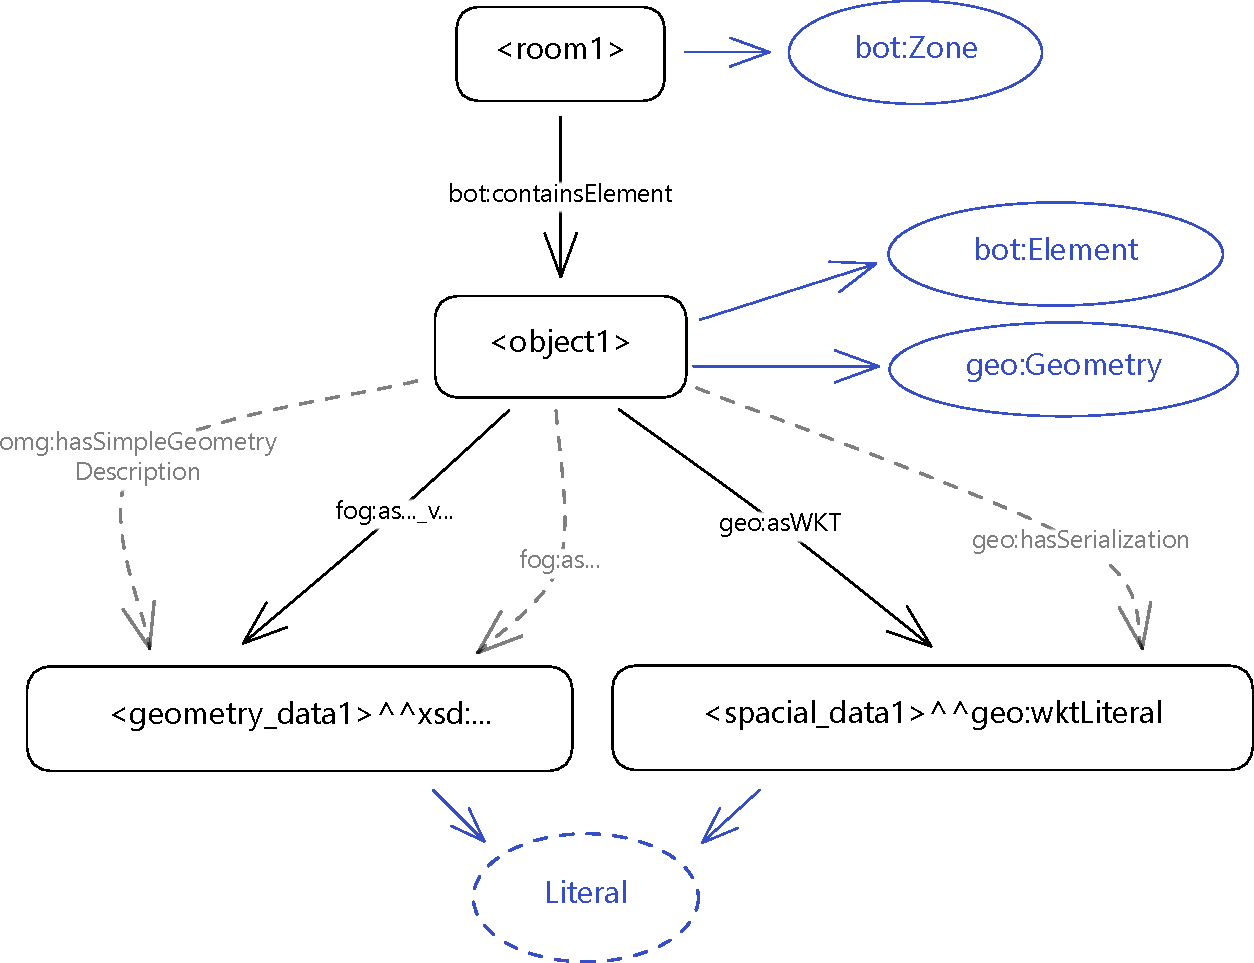
\includegraphics[width=0.8\textwidth]{figures/pdf/omg1.pdf}
    \caption[Serialization, \acs{omg} level 1]{Serialization of a geometry using the \acs{omg} level 1 pattern.}
    \label{fig:omg1}
\end{figure}


The separation into two sets allows for querying entities that have a \ac{wkt} serialization but are not located in a \mintinline{sparql}|bot:Space| (such as a floor, which would not be linked to a room) and entities that are located in a \mintinline{sparql}|bot:Space| that has a \ac{wkt} serialization. The latter variant uses the \mintinline{sparql}|bot:containsElement| or \mintinline{sparql}|bot:adjacentElement| properties to select entities within a room.

After filtering out spaces, the geometry of which is not needed by the viewer, it filters the entities' geometry based on a list of implemented/accepted formats by the receiving viewer. These last consist of a list of \ac{fog} super-properties inferred by their assignment. In other words: a triple in the \ac{rdf} graph of the form \mintinline{sparql}|?entity fog:asObj_v3.0| \mintinline{sparql}|?geometry_data| infers \mintinline{sparql}|?entity fog:asObj ?geometry_data| (as shown in Figure \ref{fig:omg1}). This allows for the use of a single property to query related formats while still permitting the declaration of more specific formats if needed.

In the end, the query returns a list of entities that are located in the same room as the observer, or are not located in a room but have a \ac{wkt} serialization that is validated by the GeoSPARQL filter function. Together with the needed metadata, which is further explained in Section \ref
{sec:interactions}.

A):
\mintinline{sparql}|?entity fog:asObj ?geometry_data|

b):
\begin{listing}[H]
    \inputminted{sparql}{dynamicQueries/inSitu/query.rq}
    \vspace{-0.7cm}
    \caption{Dynamic culling query using GeoSPARQL}
    \label{lst:GeoSPARQLauto}
\end{listing}

In the case of Listing \ref{lst:GeoSPARQLauto}, the GeoSPARQL \mintinline{sparql}|FILTER| uses the function \mintinline{sparql}|geof:sfWithin| to evaluate if the given point coordinates are within the \ac{wkt} serialization, which in most cases represents a \ac{wkt} polygon. For example:\\
\mintinline{turtle}|"POLYGON ((40 10, 30 10, 30 40, 40 40, 40 10))"^^geo:wktLiteral|

The use of GeoSPARQL results in a very efficient query, as the filtering is done directly in the query and does not require any post-processing. Although the lack of 3D capabilities is a limitation, it allows, in 2D to easily implement more complex algorithms leveraging the use of different functions. With which, together with a level 2 \ac{omg} pattern, \ac{lod} culling based on the distance to the observer can be implemented.

Selecting rooms and entities outside the room in which the observer is present is also conceivable when leveraging the use of the \mintinline{sparql}|bot:adjacentZone| property. Or using the GeoSPARQL distance to a room.
% query by distance, instance instead adjacent

\section{In viewer \enquote{bot:Space} identification} \label{sec:inViewer}
% - 1 database + 1 3D enabled instance (viewer) 
%   => viewer can raytrace identify wright space (little computation)
% - 2 layered viewer visible elements / invisible spaces
% - sequence diagram
%   - manual first step + adjacent spaces
%   - all spaces
%   - combination of spaces
% - sample queries
In this culling approach, ray tracing is employed to assess the room where the observer is situated. As illustrated in Figure \ref{fig:3participants}, out of the three participants, only one utilizes a 3D engine—a component capable of handling geometric modeling operations, such as ray tracing—referred to as the 3D viewer. In essence, both the \ac{sparql} endpoint and the external database lack the ability to perform 3D operations or evaluations. Consequently, this approach capitalizes on the 3D viewer to pinpoint the room in which the observer is positioned.

\begin{figure}[H]
    \centering
    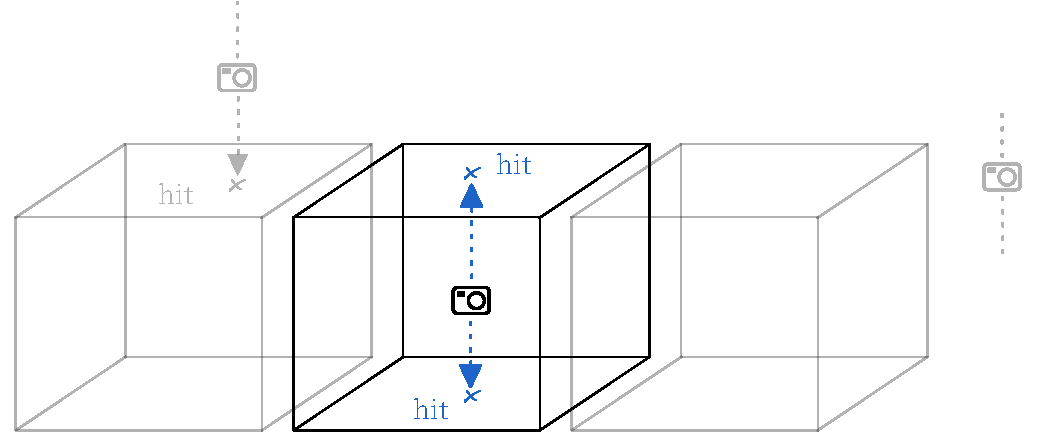
\includegraphics[width=0.8\textwidth]{figures/pdf/inViewer.pdf}
    \caption{In viewer \enquote{bot:Space} identification, with raytracing}
    \label{fig:raytrace}
\end{figure}

This process involves casting a ray from the observer's position both upwards and downwards, and evaluating the first intersection with a \mintinline{sparql}|bot:Space| entity. Unlike the previous approach, the geometry of the rooms themselves is required by the viewer, necessitating an initial query to load the rooms' geometry. By utilizing multiple layers in the viewer, the rooms' geometry can be concealed from the user while still being employed for ray tracing. Listing \ref{lst:findRoom} demonstrates the function used in this thesis prototype to assess the location. The scope of the picking is limited to the rooms using the cache's metadata, in this case \mintinline{ts}|lru: RefLRU|. Subsequently, two picking operations are carried out and compared, as depicted in Figure \ref{fig:raytrace}; if they match, the intersected room's \ac{uri} is returned.

\begin{listing}[h]
    \inputminted{ts}{dynamicQueries/inViewer/raytrace.ts}
    \vspace{-0.7cm}
    \caption{Typescript code for raytracing in viewer}
    \label{lst:findRoom}
\end{listing}

Once the room is identified, the query in Listing \ref{lst:BOTauto} is executed to retrieve the entities located within the room. This is achieved by querying the \mintinline{sparql}|bot:containsElement| property of the room. Similar to the previous method, it necessitates the combination of two sets of entities in this case: those located in the room and in the adjacent rooms themselves. This enables the optimization of the viewer by evaluating only the adjacent rooms, rather than all the rooms in the database.

The remainder of the query closely mirrors the previous one (Listing \ref{lst:GeoSPARQLauto}), with the distinction that it necessitates the additional storage of the \mintinline{sparql}|?botType| property to keep track of \ac{bot} classes and to identify \mintinline{sparql}|bot:Space| elements locally.

Due to the absence of \mintinline{sparql}|bot:adjacentZone| relations in the database used for the prototype, the query is unable to directly query the adjacent rooms. Instead, the property \mintinline{sparql}|bot:adjacentElement| is employed to query related room's adjacent walls and, consequently, the corresponding rooms. The lack of \ac{bot} relations in the utilized database was identified as a recurring issue in this thesis. Chapter \ref{ch:discussion} delves into this problem in greater detail.

This approach takes advantage of the 3D viewer and its engine to contribute to the culling process, although the first step requires downloading all the rooms' geometry. However, this step can be replaced by an initial manual localization by the user. By utilizing the adjacent rooms during subsequent queries, the impact on performance and resource usage remains minimal throughout the operation. In contrast to the \nameref{sec:inSituWKT}, this method is not limited to 2D but can be employed in 3D. However, it requires the geometry format of the room to be compatible with the viewer.

\begin{listing}[H]
    \inputminted{sparql}{dynamicQueries/inViewer/query.rq}
    \vspace{-0.7cm}
    \caption{Querying in viewer "bot:Space" identification}
    \label{lst:BOTauto}
\end{listing}

\section{In query OBJ geometry filtering} \label{sec:inQuery}
% - no geometric but string analysis in query
% - AABBox filtering of for example obj rooms
% - all negative points
This last approach is similar to the previous one, in that it also relies on the existing 3D geometry of the rooms, not their additional \ac{wkt} serialization. However, in contrast to \nameref{sec:inViewer}, the computation is once again offloaded to the \ac{sparql} endpoint. Since this endpoint is unable to perform geometric operations, a string analysis is performed instead.

The idea proposed by this thesis is to evaluate a string value, the literal representing the geometry, within a single \ac{sparql} query. As complicated string operations are difficult to perform with native \ac{sparql} functions, a custom JavaScript function is added to the \ac{sparql} endpoint. This function is then called within the query, as illustrated in Listing \ref{lst:OBJauto}. The prototype of this thesis uses GraphDB as its \ac{sparql} endpoint and \ac{rdf} database, which allows the addition of user-defined functions. Listing \ref{lst:graphdbNewFunction} demonstrates the addition of the function to the endpoint.

\begin{listing}[H]
    \inputminted{sparql}{dynamicQueries/inQuery/query.rq}
    \vspace{-0.7cm}
    \caption{Querying in query OBJ geometry filtering}
    \label{lst:OBJauto}
\end{listing}

The function itself (Listing \ref{lst:OBJautoFunction}) evaluates whether a given point is inside a geometry by extracting the vertex coordinates of the geometry literal to build an \ac{aabbox} in the form of a $3\times2$ matrix representing both a minimum and maximum value for each of the three axes. It then evaluates each point's coordinates against the given interval, returning a boolean value. The returned boolean can be interpreted by the \mintinline{sparql}|FILTER| clause inside the query, as illustrated in Listing \ref{lst:OBJauto}.

\begin{listing}[H]
    \inputminted{sparql}{dynamicQueries/inQuery/insert.rq}
    \vspace{-0.7cm}
    \caption{Inserting new javascript function in GraphDB}
    \label{lst:graphdbNewFunction}
\end{listing}

The advantages of this technique are that, similar to the previous proposal, 3D culling is achievable, there is no need for an extra serialization such as \ac{wkt}, and the computation is offloaded to the \ac{sparql} endpoint. However, the possibility to evaluate multiple geometry formats is on one side more flexible, as newer functions can interpret newer formats, not restricted by the viewer capabilities. This builds upon the concept of an all-knowing database serving a knowledge-free viewer (Section \ref{sec:proposal}). Although the possibility of allowing the JavaScript functions to fetch external files was not tested in this thesis, it could be a potential extension.

On the other hand, the function was tailored specifically for the \ac{sparql} endpoint used in this thesis, GraphDB, and would need to be adapted to other endpoints since no standard for user-defined functions was found during the research. Additionally, the JavaScript function was limited during the development of the prototype to a restricted scope of the JavaScript language, resembling the \ac{es5} version, which reduces the possibilities and optimization of the function.
\begin{listing}[H]
    \inputminted{js}{dynamicQueries/inQuery/function.js}
    \vspace{-0.7cm}
    \caption{Querying in situ WKT location}
    \label{lst:OBJautoFunction}
\end{listing}


\chapter{Modular Approach} \label{ch:modularApproach}
This chapter describes a theoretical modular approach for the implementation of this thesis' proposed \ac{ldbim} viewer and associated culling techniques. This design principle consists of separate, independent modules, with each module responsible for a specific functionality of the framework. They are designed to be compatible with any web development framework. The modular approach is important for the following reasons:

\begin{itemize}
    \item \textbf{Extendability}: The modular approach makes it easy to extend the framework with new functionalities, allowing for the addition of new features without altering existing ones.
    \item \textbf{Maintainability}: Modules form meaningful units, making it easy to maintain and update the framework. The structure is easily readable, enabling targeted updates or maintenance efforts.
    \item \textbf{Reusability}: The reusability of modules allows them to be implemented in other projects. This section proposes the role each module should have in the framework, facilitating extrapolation to other web development frameworks.
\end{itemize}

The modules are designed to be specific to both the culling and the \ac{ldbim} viewer. The theoretical model proposed in this thesis is informed by practical experiences and observations gained through the development of the prototype.

The main module, the viewer, and its requirements (Section \ref{sec:viewerRequirements}) have already been discussed in Chapter \ref{ch:dynamicQueries}.

\section{Data fetching}
This section discusses the modules responsible for retrieving external data. Two submodules can be identified: the \ac{sparql} fetcher and the database fetcher. The \ac{sparql} fetcher handles communication with the \ac{rdf} database and \ac{sparql} endpoint, while the database fetcher manages communication with external databases where geometry files may be stored. The primary function of these modules, with respect to data fetching, involves authentication and error handling for requests.

Authentication and error handling are crucial when facilitating communication between multiple web instances, such as the website, database, and \ac{sparql} endpoint. By incorporating these functionalities into separate modules, the framework can be adapted to suit the requirements of each use case. This allows for different authentication methods and error handling procedures to be employed, depending on the technology used by each web instance.

\subsection{\acs{sparql} fetcher}
The \acs{sparql} fetcher module handles the back and forth communication with the \ac{rdf} database and \ac{sparql} endpoint. It should do this in two situations:

\begin{itemize}
    \item When the \ac{sparql} query is updated, the module fetches the results of the query from the \ac{sparql} endpoint. This includes the metadata of every given entity provided by the \ac{sparql} endpoint for the cache manager.
    \item When the entities are approved by the cache manager, the module fetches the geometry literals from the \ac{rdf} database, via the \ac{sparql} endpoint.
\end{itemize}

As mentioned above, the \ac{sparql} fetcher retrieves data from the \ac{sparql} endpoint and is not an endpoint itself. This is done to offload the querying from the viewer, which is a resource-intensive task. It also implies that this module is responsible for the authentication of the connection, error handling, and result interpretation. Metadata about entities is dispatched from this module to the cache manager, waiting for approval before a new query is sent for the retrieval of geometry literals. Once loaded, these literals are dispatched to the viewer for rendering.

Serving two main functions but only communicating with one web instance, the choice was made to combine the two functions into one module. This allows for sharing the same authentication and error handling procedures.

\subsection{Database fetcher} \label{sec:databaseFetcher}
This module, triggered by the cache manager, retrieves the geometry files from an external file server or database. Similarly to the \ac{sparql} fetcher, it is responsible for authentication and error handling. It is also responsible for the interpretation of the results, dispatching the geometry files to the viewer for rendering.

\section{Cache manager}
The cache manager is responsible for managing the cache. It is the module that decides which entities are to be cached, and which are to be removed from the cache to subsequently be removed from the viewer. This module is crucial for the performance of the framework, as it determines which entities are to be added and which are to be removed from the viewer. It is also responsible for maintaining the integrity of the metadata about entities in the viewer, ensuring that the cache is not filled with outdated metadata.

Therefore, it evaluates if results from the \ac{sparql} fetcher already exist in the viewer/cache, and if so, whether they are up-to-date. If the results are not up-to-date or propose a new entity, the cache manager will trigger the fetching of the new geometry by the appropriate fetcher. The cache manager is also responsible for keeping track of the entities in the viewer and removing them when they are no longer relevant.

This last functionality requires the use of a cache replacement algorithm. The algorithm determines which entities are to be removed from the viewer, based on a set of rules such as: the number of entities in the viewer, the time since the entity was last viewed, the number of times the entity was viewed, etc. To illustrate the functionality, the following section will discuss the \ac{lru} algorithm. This algorithm was chosen because of its simplicity and ease of implementation. It is also a popular algorithm for cache replacement and is therefore a good starting point for the development of the framework. Some other possible algorithms are, for example, the \ac{lfu}, \ac{fifo}, \ac{lifo}, and \ac{mru} algorithms\parencite{cacheAlgorigthms}. These algorithms are not discussed in this thesis but are possible candidates for future research, as they may be better suited for the proposed framework.

\subsection{\acs{lru} algorithm}
As a possible cache replacement algorithm, the \ac{lru} algorithm limits the number of entities allowed in the viewer. It can be interpreted as a list in which new entities are added at the front of the list, and existing entries are repositioned at the front. Whenever a new entity is added to the list, it causes the current entities to move further down the list. If an already-existing entity is accessed again, it gets moved up to the front of the list, but this doesn't cause any change to the position of the entities at the tail of the list. When the list is full, the entity at the end of the list is removed from the viewer, as it is the least recently used entity \parencite{cacheAlgorigthms}.

To implement this algorithm, the cache manager needs to store the metadata of each new entity, or if the entity already exists, compare the new metadata and move it to the front of the list, triggering the fetching modules.

\section{Query processing}
The query processing module proposed by this thesis comprises multiple submodules, aiming to assemble the \ac{sparql} query from different sources, such as the \ac{ui}, culling algorithm, and other user-specific settings.

\subsection{Query builder}
To facilitate the construction of the \ac{sparql} query, the query builder module is responsible for assembling the query from the different requirements stated by the culling algorithms. Thereby constructing a query that complies with the various algorithms in one. It concatenates the abstractions stated by these algorithms into one coherent query, reducing the load on the \ac{sparql} fetcher.

The sub-functions or culling algorithms of this module need access to the rest of the framework. As illustrated in Sections \ref{sec:inSituWKT}, \ref{sec:inViewer}, and \ref{sec:inQuery}, it will require communication with the viewer to retrieve the camera position and execute 3D operations.

\subsection{Query composer}
As the \ac{ui} interactions can override the query generated by the building module, the query composer module is responsible for combining the query from the query builder with the query parameters from the \ac{ui}. Performing a final check on the query, it ensures that the query is valid and ready to be sent to the \ac{sparql} fetcher.

By separating this module from the builder, the builder can focus on the construction of the culling query, while the composer can concentrate on the combination of the query with the \ac{ui} parameters independently of the culling query.

\section{Interactions} \label{sec:interactions}
All the modules are joined together in one flexible framework illustrated in Figure \ref{fig:interactionModules}. Four main modules create the proposed framework. The query processing module, once fed with data from both the cache manager and viewer, concatenates the different submodules to the query composer, creating a \ac{sparql} query. This query creation triggers a first request to the \ac{sparql} endpoint, which returns metadata about the needed entities. Once approved by the cache manager, to avoid constantly reloading the geometry data, it gets dispatched to the \ac{sparql} or database fetcher. The retrieved geometry data is then sent to the viewer for rendering. Afterwards, the cycle starts again, feeding viewer and cache manager data to the dynamic culling query algorithms.

\begin{figure}[H]
    \centering
    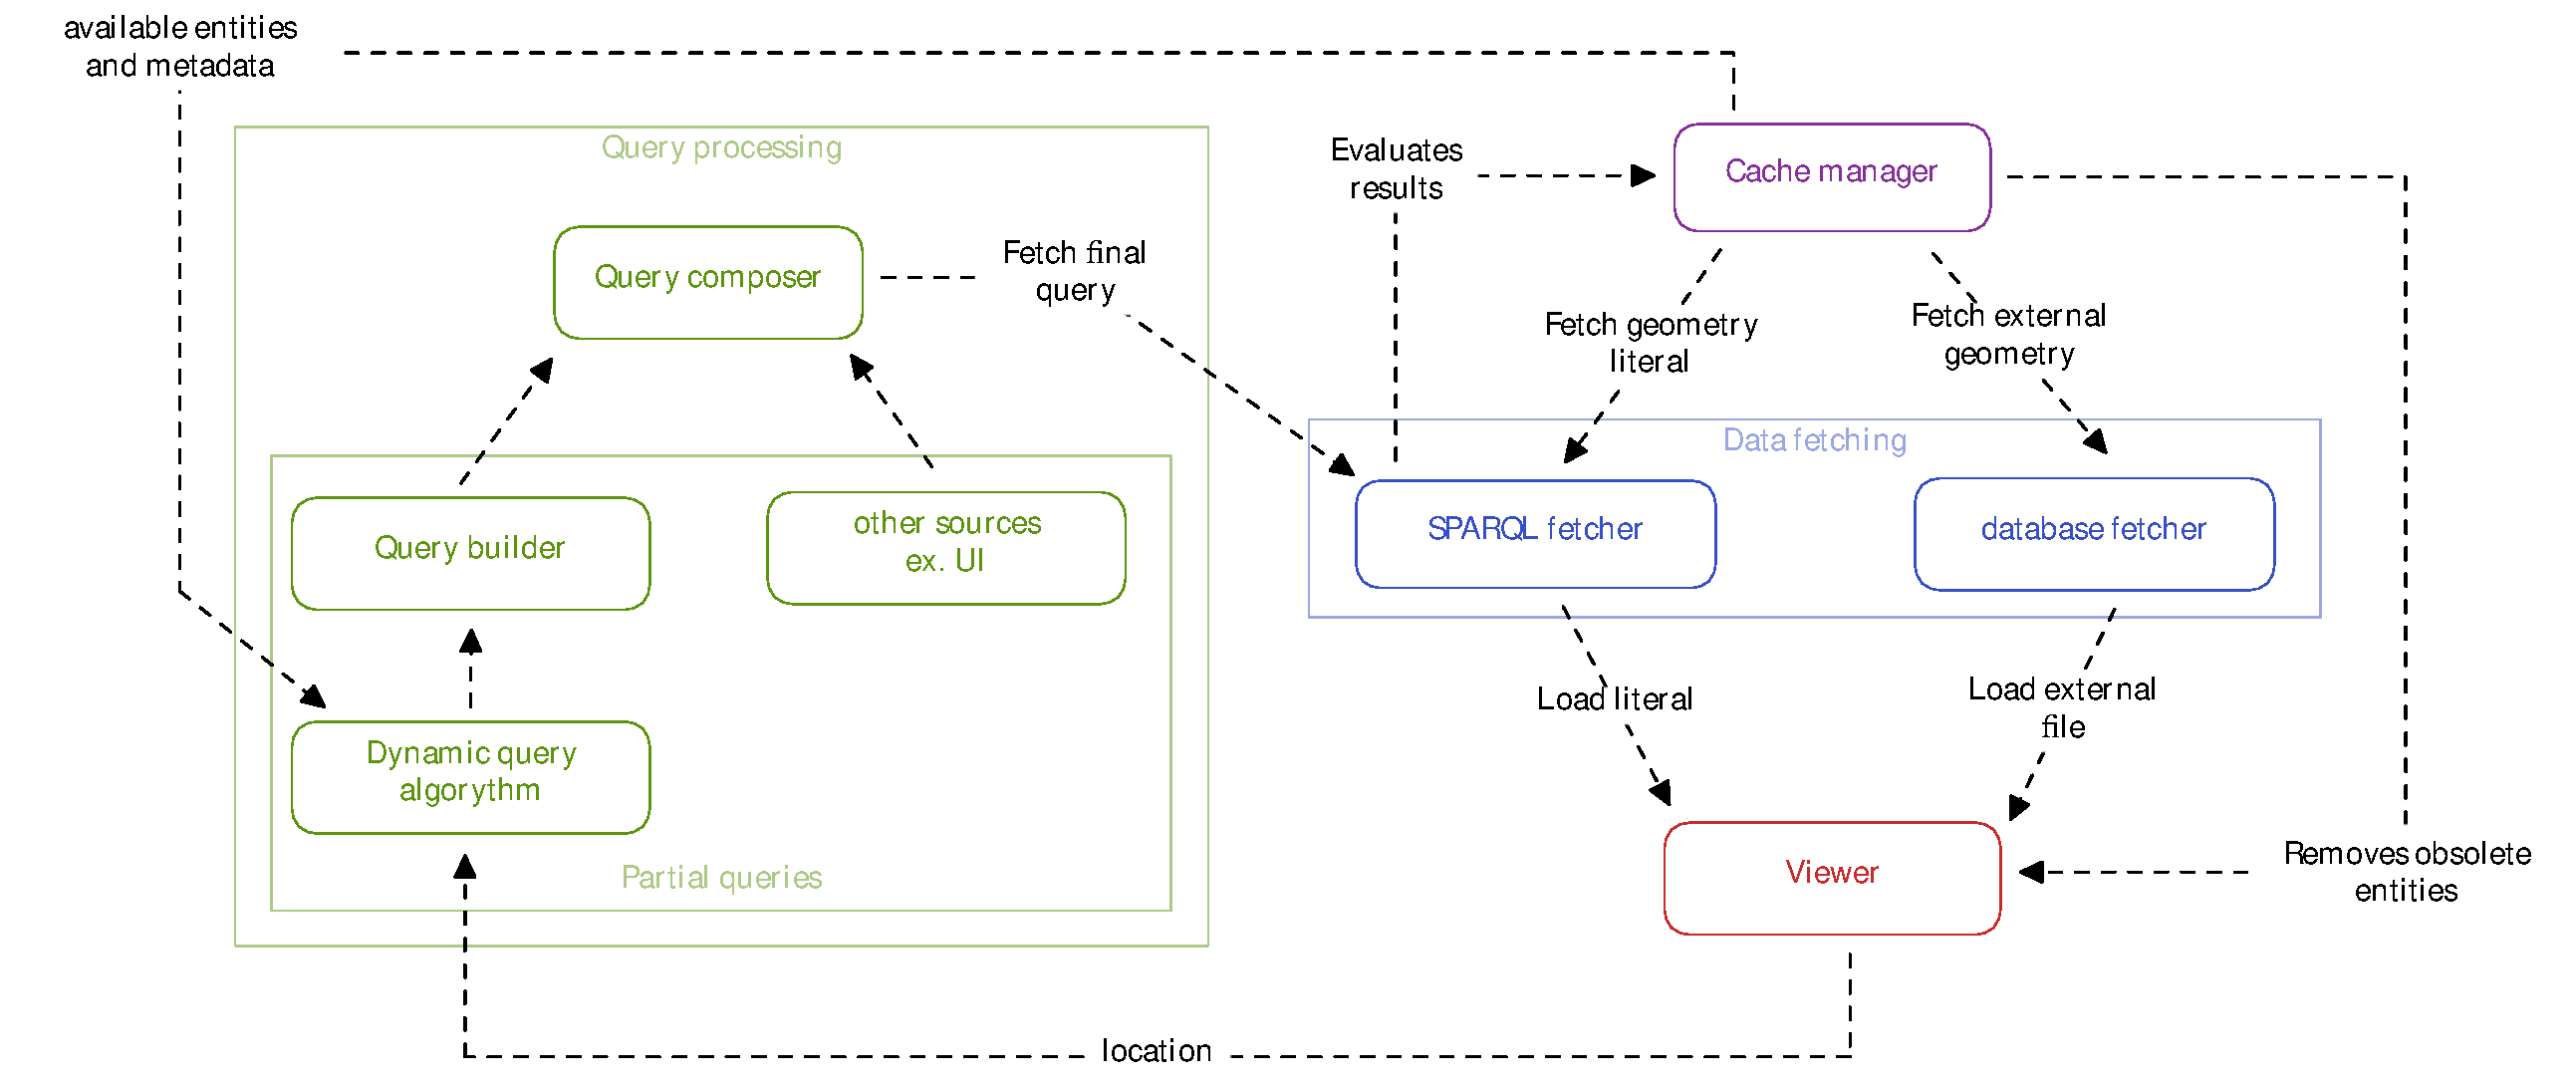
\includegraphics[width=\textwidth]{figures/pdf/interactions_concept.pdf}
    \caption[Interactions modular framework]{Conceptual diagram of the interactions between the modules.}
    \label{fig:interactionModules}
\end{figure}

\chapter{Prototype} \label{ch:prototype}
The code for the prototype developed in this thesis is available at:\\
\url{https://github.com/flol3622/LDBIM-viewer}.

\section{Database design}
The database used in this thesis is based on the database developed by Mads Holten Rasmussen and made available at:\\
\url{https://github.com/MadsHolten/BOT-Duplex-house/tree/master/Model%20files/LBD}

It was chosen as a starting point, as it already contained \ac{bot} descriptions and relations between entities which are heavily utilized by this thesis' algorithm. Additionally, it was selected because it already contained geometry descriptions of those entities. As well as containing \ac{wkt} serializations of walls, rooms, and floor entities. Although the size of the model it describes is small, too small to evaluate culling performance, no other suitable database meeting the requirements was found.

Nevertheless, some changes had to be made to accommodate the needs of this thesis. This section will describe these changes.

\subsection{GraphDB}
To host the database, and exercise the role of the \ac{sparql} endpoint, a GraphDB instance was run locally to store, query, modify, and extract the semantic data. \enquote{GraphDB is an enterprise ready Semantic Graph Database, compliant with W3C Standards}\footcite{graphdb} It was chosen for its simple installationa and application, its support for the GeoSPARQL extension (Section \ref{sec:inSituWKT}), as well as the possibility to create custom functions in JavaScript (Section \ref{sec:inQuery}).

To comply with the requirements of the algorithm, the structure of the database had to be altered to resemble the one illustrated in Figure \ref{fig:omg1}. Figure \ref{fig:dbadaptation} illustrates the changes made to the database, where the existing data was used to describe new relations needed for this thesis.

\begin{figure}[H]
    \centering
    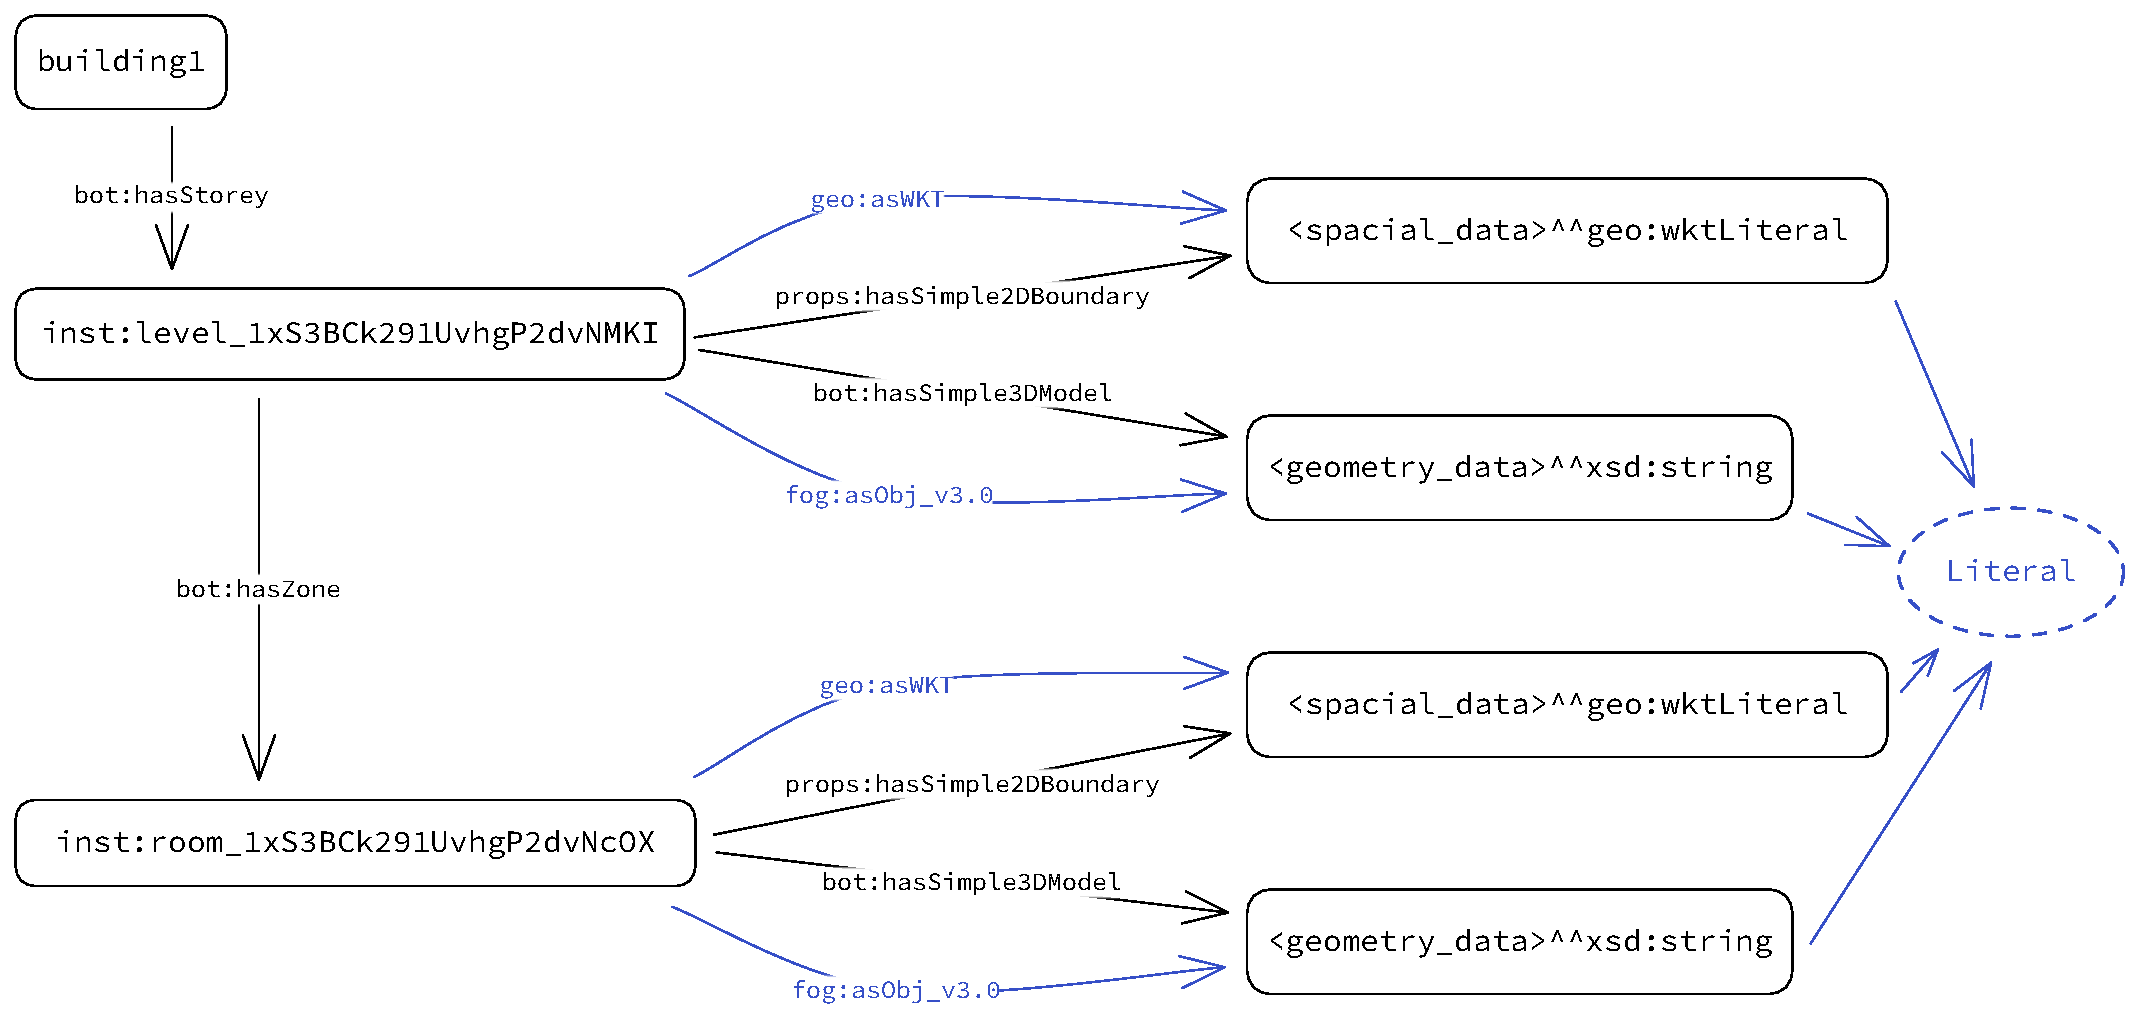
\includegraphics[width=\textwidth]{figures/pdf/dbadaptation.pdf}
    \caption[Database adaptation]{Database adaptation to Figure \ref{fig:omg1}.}
    \label{fig:dbadaptation}
\end{figure}

\subsection{3D geometries}
Listing \ref{lst:insertFOG} demonstrates how the \ac{fog} ontology was implemented in the \ac{rdf} database. The following subsections describe the additional steps taken to adapt the database to the specific requirements of the viewer used.

\begin{listing}[H]
    \begin{minted}{sparql}
PREFIX bot: <https://w3id.org/bot#>
PREFIX fog: <https://w3id.org/fog#>

INSERT { ?s fog:asObj_v3.0 ?o . }
WHERE { ?s bot:hasSimple3DModel ?o . }
    \end{minted}
    \caption[Inserting \acs{fog} relations]{Inserting \acs{fog} relations into the database.}
    \label{lst:insertFOG}
\end{listing}

\subsubsection{Extracting geometries from \ac{rdf} database}
Due to the inability to display OBJ literals in the utilized viewer, the geometries had to be extracted from the database and stored as separate files. This was accomplished using a Python script (Appendix \ref{sec:pyhtonExtraction}), which extracted the geometries from the database using Listing \ref{lst:extractGeometries} and stored them as separate files.

\begin{listing}[H]
    \begin{minted}{sparql}
SELECT ?s ?o
WHERE {
    SERVICE <http://localhost:7200/repositories/duplex-v1> {
    ?s fog:asObj ?o .
    filter(datatype(?o)=xsd:string)
    }
}
    \end{minted}
    \caption{\acs{sparql} query to extract geometries.}
    \label{lst:extractGeometries}
\end{listing}


\subsubsection{Rescaling geometries}
Rescaling the entities to fit the viewer's coordinate system was executed by using the open-source 3D modeling software, Blender. This software allowed for the batch import, rescale, and export of the different entities. However, batch export into multiple files was restricted to the STL file format only. After which, the individual files were uploaded to the \href{https://github.com/flol3622/LDBIM-viewer}{GitHub repository} of the prototype, which functioned as an external database.

\subsubsection{Inserting data}

The new external files were inserted in the database using the \ac{sparql} query in Listing \ref{lst:insertLinks}. This query designated the literal's datatype as \mintinline{turtle}|xsd:anyURI| (Section \ref{sec:fog}), which the prototype would later use to treat the resource as a link to an external file (Section \ref{sec:databaseFetcher}).

\begin{listing}[H]
    \begin{minted}{sparql}
PREFIX fog: <https://w3id.org/fog#>
PREFIX xsd: <http://www.w3.org/2001/XMLSchema#>

INSERT { ?s fog:asStl_v1.0-ascii ?newURI }
WHERE { 
    ?s fog:asObj_v3.0 ?o .
    FILTER (datatype(?o) = xsd:anyURI)
    BIND (REPLACE(STR(?s), "https://172.16.10.122:8080/projects/1001/", "") AS ?localName)
    BIND (REPLACE(STR(?localName), "%", "-") AS ?newLocalName)
    BIND (CONCAT("https://raw.githubusercontent.com/flol3622/LDBIM-viewer/main/public/assets/duplex-v1/stl_m/", ?newLocalName, ".stl") AS ?uriString)
    
    BIND (STRDT(?uriString, xsd:anyURI) AS ?newURI)
}
    \end{minted}
    \caption{Inserting external links with \acs{fog}}
    \label{lst:insertLinks}
\end{listing}

\subsection{\acs{wkt} serialisation}

Similarly to the geometries, the \ac{wkt} literals were implemented using the GeoSPARQL ontology, as shown in Listing \ref{lst:insertWKT}.

\begin{listing}[H]
    \begin{minted}{sparql}
PREFIX props: <https://w3id.org/props#>
PREFIX geo: <http://www.opengis.net/ont/geosparql#>

INSERT { ?s geo:asWKT ?o . }
WHERE{ ?s props:hasSimple2DBoundary ?o . }
    \end{minted}
    \caption[Inserting \acs{wkt} literals]{Inserting \acs{wkt} literals using GeoSPARQL.}
    \label{lst:insertWKT}
\end{listing}

\subsubsection{Syntax correction}

A Python script was created (see Appendix \ref{sec:wktVisualisation}) to experiment with the \ac{wkt} literals. This script visualized the \ac{wkt} literals using the matplotlib package. This revealed syntax errors in the \ac{wkt} literals, which were corrected using the query in Listing \ref{lst:fixWKT}, to enable the use of GeoSPARQL functions. The query modifies the \ac{wkt} literals from the format: \mintinline{turtle}|"POLYGON (x1 y1, x2 y2 ,...)"^^geo:wktLiteral| to:\\
\mintinline{turtle}|"POLYGON ((x1 y1, x2 y2 ,...))"^^geo:wktLiteral|. The adjustment adds an extra pair of parentheses to the POLYGON definition, adhering to the correct syntax for a \ac{wkt} Polygon literal, as defined by the GeoSPARQL standard.

\begin{listing}[H]
    \begin{minted}{sparql}
PREFIX geo: <http://www.opengis.net/ont/geosparql#>

DELETE { ?room geo:asWKT ?old_wkt . }
INSERT { ?room geo:asWKT ?new_wkt . }
WHERE {
    ?room geo:asWKT ?old_wkt .
    BIND(str(?old_wkt) as ?old_lit)
    FILTER (
        STRSTARTS(?old_lit, "POLYGON (") &&
        !STRSTARTS(?old_lit, "POLYGON ((")
    )
    BIND (STRDT(CONCAT("POLYGON (", SUBSTR(?old_lit, 9), ")"), geo:wktLiteral) AS ?new_wkt
    )
}
    \end{minted}
    \caption{Fixing \acs{wkt} syntax.}
    \label{lst:fixWKT}
\end{listing}

\section{Web Development Stack}
The prototype was developed using the \href{https://nextjs.org/}{Next.js framework}, which is built on top of React, a popular JavaScript library for building component-based web applications. This choice adheres to the modular approach explained in Chapter \ref{ch:modularApproach}. Next.js and the following tools or libraries were chosen for their popularity and ease of use within the React ecosystem:

\begin{itemize}
    \item \href{https://recoiljs.org/}{Recoil:} As a state management library, Recoil was used to manage and exchange data between the different modules. It provides a simple and efficient way to share state across components.

    \item \href{https://tailwindcss.com/}{Tailwind CSS:} Adopted for styling the \ac{ui} components, Tailwind CSS facilitates rapid prototyping and easy customization of the \ac{ui}.

    \item \href{https://icons.radix-ui.com/}{Radix Icons:} The Radix Icons library provided the icons used in the \ac{ui} components.

    \item \href{https://mui.com/}{Material UI:} This popular React \ac{ui} library was employed for the more complex \ac{ui} components. Material UI offers a large library of pre-built components that are easy to use and customize, aligning with the best practices for web \ac{ui} design.
\end{itemize}

\subsection{Specialized packages}
\subsubsection{lru\_map}
The efficient \ac{lru} algorithm used in the caching algorithm is the \href{https://github.com/rsms/js-lru}{lru\_map} package by Rasmus Andersson. This package was chosen for its simplicity and efficiency, as it implements a double-linked list which prevents the need for shifting the list when an item is accessed. This reduces the load on the lightweight viewer, ensuring optimal performance.

\subsubsection{fetch-sparql-endpoint}
The \href{https://github.com/rubensworks/fetch-sparql-endpoint.js}{fetch-sparql-endpoint} package, developed by Ruben Taelman, a Web postdoctoral researcher at IDLab, Ghent University – imec \footcite{RubenTaelman}, is used in the prototype's \ac{sparql} fetcher module to manage communication with the \ac{sparql} endpoint. This package facilitates the process of sending queries to, and receiving responses from the endpoint, providing a simple and effective way to interact with the \ac{rdf} database.

\subsection{Xeokit-\acs{sdk}}
Following \cite{Malcolm2021} and their \ac{lbd} Server, the prototype of this thesis utilizes the \href{http://xeokit.io/index.html}{Xeokit SDK}, described as an \enquote{open source 3D graphics SDK from xeolabs for BIM and AEC}\footcite{xeokit}. This \ac{sdk} supports an extensive array of 3D formats employed in the \ac{aec} industry, as detailed in Table \ref{tab:xeokitFormats}. It also supplies the necessary tools to construct the viewer module in accordance with the requirements described in Section \ref{sec:viewerRequirements}.

\begin{table}[H]
    \centering
    \begin{tabular}{lll}
        \toprule
        BCF Viewpoints & IFC & GLTF \\
        CityJSON       & OBJ & STL  \\
        3DXML          & XKT & LAS  \\
        \bottomrule
    \end{tabular}
    \caption[Supported formats in Xeokit \acs{sdk}]{Supported formats in Xeokit \acs{sdk}.\footnotemark}
    \label{tab:xeokitFormats}
\end{table}
\footnotetext{\cite{xeokit}}

\section{Structure}
The prototype's design, translated into the conceptual modular approach discussed in Chapter \ref{ch:modularApproach}, is depicted in Figure \ref{fig:interactionPrototype}. The four main modules are further dissected into components developed using the previously mentioned tools and libraries. These fall into one of three categories:

\begin{itemize}
    \item \textbf{React components:} The \ac{ui} components that are rendered in the browser. They display output elements and/or receive user input.
    \item \textbf{React hooks:} The functions used to manage the state of the application. They store and update data, which is passed on to the React components.
    \item \textbf{JavaScript functions:} Standalone functions used to perform specific tasks, such as fetching or computing data.
\end{itemize}

In the case of the GeoSPARQLauto module, which executes a culling technique based on the \ac{wkt} serialization as proposed in Section \ref{sec:inSituWKT}, the query processing module receives localisation data from the viewer module. This data passes through the useAutomations hook, which manages the different culling algorithms. The QueryPanel component allows selection between the culling algorithms and the user-defined query from the QueryInput component. This selector stores the final query, which triggers the useLoadGeometry hook from the viewer module. This hook uses the getEntities function to fetch data from the \ac{sparql} endpoint, which then communicates with the evalLRU function from the cache manager for entity approval. Upon approval, the useLoadGeometry hook fetches the geometry data using the getGeometry function, retrieving a geometry literal or an \ac{uri}. The hook then send it to the viewer for loading into the scene. The loading occurs within Xeokit's loading plugins, which accept literal values or \ac{uri}s and fetch the external files independently. Once all the entities are loaded, the viewer's scene is compared to the updated \ac{lru} list, using the syncViewer function to remove obsolete entities.

\begin{figure}[H]
    \centering
    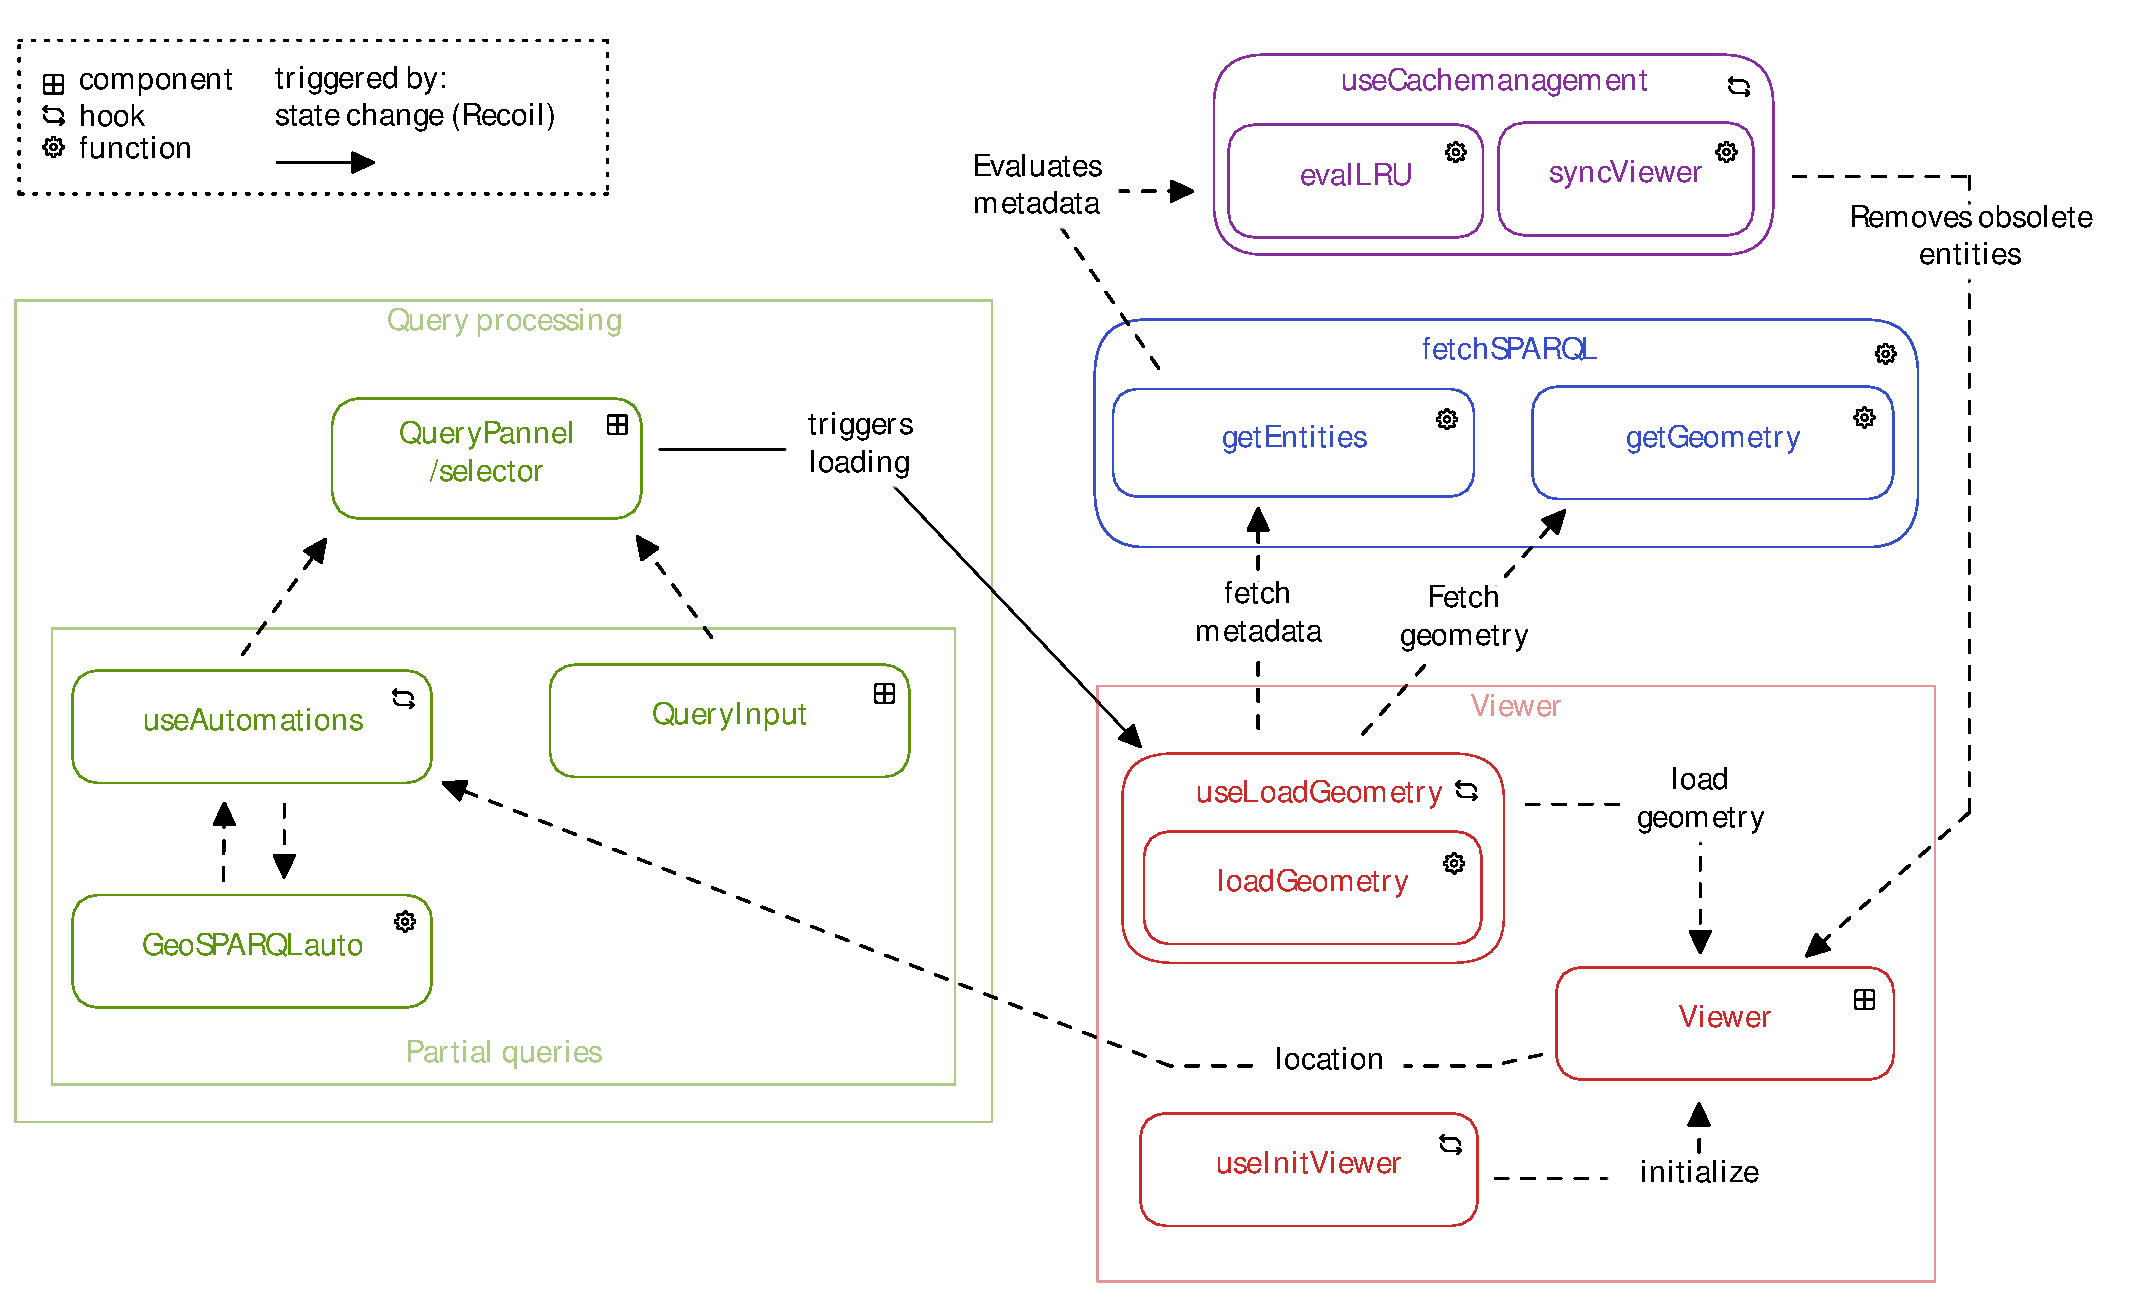
\includegraphics[width=\textwidth]{figures/pdf/interactions_prototype.pdf}
    \caption[Interactions prototype]{Conceptual diagram of the interactions between the modules within the prototype when using a dynamic query algorithm, such as GeoSPARQLauto, based on Figure \ref{fig:interactionModules}.}
    \label{fig:interactionPrototype}
\end{figure}

\section{Semantic visualisation} \label{sec:semanticVis}
\begin{listing}[H]
    \inputminted{ts}{dynamicQueries/colorize/type.ts}
    \caption[\acs{lru} entry type]{Type of the \ac{lru} entries, extendible to include additional metadata.}
    \label{lst:lruType}
\end{listing}

The cache management module is constructed in such a way that the \ac{lru} list stores metadata about the entities. Each entry in the cache management module is stored with a unique identifier, represented by its \ac{uri}. This identifier serves as the key for each entry. Correspondingly, the value of each entry is represented as a JavaScript object. As of the current state of the prototype, this object contains details such as the datatype and the format of the geometry. Therefore, this object can be extended to accommodate properties such as the non-geometrical ones described in Section \ref{sec:beyondGeometry}, as illustrated in its type description in Listing \ref{lst:lruType}.

\begin{listing}[H]
    \inputminted{json}{dynamicQueries/colorize/entry.json}
    \caption[LRU entry]{Example of an entry in the \ac{lru} list.}
    \label{lst:lruEntry}
\end{listing}

To illustrate this proposal, a triple containing color data was inserted into the database, with the query used shown in Listing \ref{lst:colorInsert}. The entry in Listing \ref{lst:lruEntry} displays the metadata stored in the \ac{lru} list for this entity. The color data is then applied to the geometry using the Xeokit \ac{api}. Since the latter does not allow color assignment during entity loading, the color is applied after the entity is loaded, within the syncViewer function (see Appendix \ref{sec:cache.ts}).

\begin{listing}[H]
    \inputminted{sparql}{dynamicQueries/colorize/insert.rq}
    \caption[Insert color data]{Insertion of color data into the database.}
    \label{lst:colorInsert}
\end{listing}

\section{Functionalities and Demonstration}
The main features of the prototype are available at:\\
\url{https://github.com/flol3622/Pre-culling_LDBIM#demo}\\
The following features were presented:

\begin{itemize}
    \item \textbf{Basic use case:} The basic use case is presented where the entire building is loaded with a maximum number of entities set to 20. The user can navigate through the building and entities are loaded on demand. The user can also change the maximum number of entities to be loaded at once.
    \item \textbf{Different sources and formats:} The prototype can load different sources and formats. A database of abstract shapes is selected which holds STL, OBJ and GLTF geometry files as literals or as links to external files on GitHub. (Section \ref{sec:viewerRequirements})
    \item \textbf{Semantic-driven filtering:} With the aid of semantics, the user can filter the entities to load in the viewer. This example filters the entities to only show the ones with \mintinline{sparql}|rdf:type prod:Window|.
    \item \textbf{Semantic-driven colorization:} Semantics associated with each entity can be used to colorize the entities in the viewer. This example colorizes the entities based on their \mintinline{sparql}|flupke:color| property which holds a color code. (Sections \ref{sec:visualSemantic}, \ref{sec:semanticVis})
    \item \textbf{In-query, OBJ-string analytics} A first culling algorithm is showcased where the \mintinline{sparql}|bot:Space| entities are filtered based on their OBJ definition, which is analyzed by the endpoint using a string operation. The cache management mechanism is also visualized as the viewer's scene does not exceed an entity count of 20. (Section \ref{sec:inQuery})
    \item \textbf{In situ, GeoSPARQL} This second culling algorithm uses GeoSPARQL functions. As the GeoSPARQL functions are limited to 2D space, the viewer hovering over a \mintinline{sparql}|bot:Space| triggers the loading of this last. (Section \ref{sec:inSituWKT})
\end{itemize}

The source code is available at: \url{https://github.com/flol3622/LDBIM-viewer}

\chapter{Conclusion} \label{ch:conclusion}
% - fact that position is known, not all 3d viewers, look at AR, aknowledge the problems remaining there

\newgeometry{bottom=2.5cm,top=-0.6cm,left=2.5cm,right=2.5cm}
\printbibliography[nottype=online, heading=bibintoc,title={References}]
\printbibliography[type=online, heading=bibintoc, title={Referenced websites}]
\restoregeometry

\appendix
\chapter{Prototype}
\label{appendix:prototype}
\pagenumbering{roman}
\setlength{\DTbaselineskip}{14pt}

\begin{footnotesize}
    \dirtree{%
        .1 src/.
        .2 components/.
        .3 index.ts.
        .3 Viewer.tsx.
        .3 Navbar.tsx.
        .3 QueryPannel.tsx.
        .3 Queryinput.tsx.
        .3 Divider.tsx.
        .3 Button.tsx.
        .2 modules/.
        .3 atoms/.
        .4 index.ts.
        .4 cleanStart.ts.
        .4 endpoint.ts.
        .4 query.ts.
        .4 lru.ts.
        .4 ui.ts.
        .3 automations/.
        .4 index.ts.
        .4 \hyperref[sec:useAutomations.ts]{useAutomations.ts}.
        .4 \hyperref[sec:BOT.ts]{BOT.ts}.
        .4 \hyperref[sec:GeoSPARQL.ts]{GeoSPARQL.ts}.
        .4 \hyperref[sec:OBJ.ts]{OBJ.ts}.
        .3 viewer/.
        .4 index.ts.
        .4 types.ts.
        .4 useInitViewer.ts.
        .4 useLoadGeometry.ts.
        .3 fetchSPARQL.ts.
        .3 \hyperref[sec:cache.ts]{useCacheManagement.ts}.
        .3 refTypes.ts.
        .2 pages/.
        .3 index.tsx.
    }
\end{footnotesize}

\section{automations}
\subsection{useAutomations}
\label{sec:useAutomations.ts}
\inputminted{ts}{figures/snippets/src/modules/automations/useAutomations.ts}
\newpage
\subsection{BOT}
\label{sec:BOT.ts}
\inputminted{ts}{figures/snippets/src/modules/automations/BOT.ts}
\subsection{GeoSPARQL}
\label{sec:GeoSPARQL.ts}
\inputminted{ts}{figures/snippets/src/modules/automations/GeoSPARQL.ts}
\newpage
\subsection{OBJ}
\label{sec:OBJ.ts}
\inputminted{ts}{figures/snippets/src/modules/automations/OBJ.ts}
\section{useCacheManagement}
\label{sec:cache.ts}
\inputminted{ts}{figures/snippets/src/modules/useCacheManagement.ts}

\chapter{Python scripts}

\section{\acs{wkt} visualisation}
\label{sec:wktVisualisation}
\begin{minted}{python}
import matplotlib.pyplot as plt
import rdflib

levels = [
    "inst:level_1xS3BCk291UvhgP2dvNMKI",
    "inst:level_1xS3BCk291UvhgP2dvNMQJ",
    "inst:level_1xS3BCk291UvhgP2dvNsgp",
    "inst:level_1xS3BCk291UvhgP2dvNtSE"
]

data = {}

for level in levels:
    g = rdflib.Graph()
    qres = g.query("""
      PREFIX props: <https://w3id.org/props#>
      PREFIX rdf: <http://www.w3.org/1999/02/22-rdf-syntax-ns#>
      PREFIX bot: <https://w3id.org/bot#>
      PREFIX inst: <https://172.16.10.122:8080/projects/1001/>
      SELECT ?s ?o
      WHERE {
        SERVICE <http://localhost:7200/repositories/duplex-v1> {
          ?s props:hasSimple2DBoundary ?o .
          ?s rdf:type bot:Space .
          """ + str(level) + """ bot:hasSpace ?s.
        }
      }
      LIMIT 100
      """)
    rooms = {}
    for row in qres:
        polygon_string = row.o.n3()
        polygon_string = polygon_string.replace('POLYGON (', '').replace('()', '').replace(')', '').replace(
            '"', '').replace('^^<http://www.opengis.net/ont/geosparql#wktLiteral>', '')
        coordinate_pairs = polygon_string.split(', ')
        coordinates = [(int(pair.split(' ')[0]), int(pair.split(' ')[1]))
                       for pair in coordinate_pairs]
        row.o.n3()
        room = row.s.n3().replace(
            '<https://172.16.10.122:8080/projects/1001/', '').replace('>', '')
        rooms[room] = coordinates
    data[level] = rooms


def showLevel(level):
    level = data[level]
    plt.figure()
    for room, polygon in level.items():
        xs, ys = zip(*polygon)
        plt.plot(xs, ys, label=room)
    plt.axis('equal')
    plt.legend(bbox_to_anchor=(1, 1))
    plt.show()
\end{minted}

\begin{minted}{python}
for level in levels:
    print(level)
    print(data[level].keys())
    showLevel(level)
\end{minted}

\begin{minted}[bgcolor=white]{output}
texttt{inst:level_1xS3BCk291UvhgP2dvNMKI
dict_keys(['room_1xS3BCk291UvhgP2dvNvkw', 'room_1xS3BCk291UvhgP2dvNvk7', 'room_1xS3BCk291UvhgP2dvNvk0', 'room_1xS3BCk291UvhgP2dvNvkD', 'room_1xS3BCk291UvhgP2dvNcNR', 'room_1xS3BCk291UvhgP2dvNcOa', 'room_1xS3BCk291UvhgP2dvNcOX', 'room_1xS3BCk291UvhgP2dvNcOY', 'room_1xS3BCk291UvhgP2dvNb9h', 'room_1xS3BCk291UvhgP2dvNbEa'])}
\end{minted}

\begin{figure}[H]
  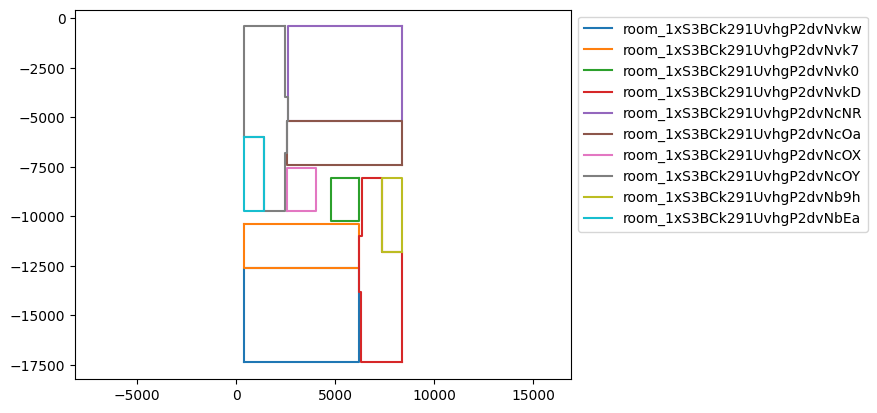
\includegraphics[width=\textwidth]{figures/png/WKT output/output1.png}
\end{figure}

\begin{minted}[bgcolor=white]{output}
inst:level_1xS3BCk291UvhgP2dvNMQJ
dict_keys(['room_1xS3BCk291UvhgP2dvNvkK', 'room_1xS3BCk291UvhgP2dvNvkG', 'room_1xS3BCk291UvhgP2dvNvkT', 'room_1xS3BCk291UvhgP2dvNvkU', 'room_1xS3BCk291UvhgP2dvNcOe', 'room_1xS3BCk291UvhgP2dvNcOq', 'room_1xS3BCk291UvhgP2dvNcOn', 'room_1xS3BCk291UvhgP2dvNcOo', 'room_1xS3BCk291UvhgP2dvNdjF', 'room_1xS3BCk291UvhgP2dvNdjS'])
\end{minted}

\begin{figure}[H]
  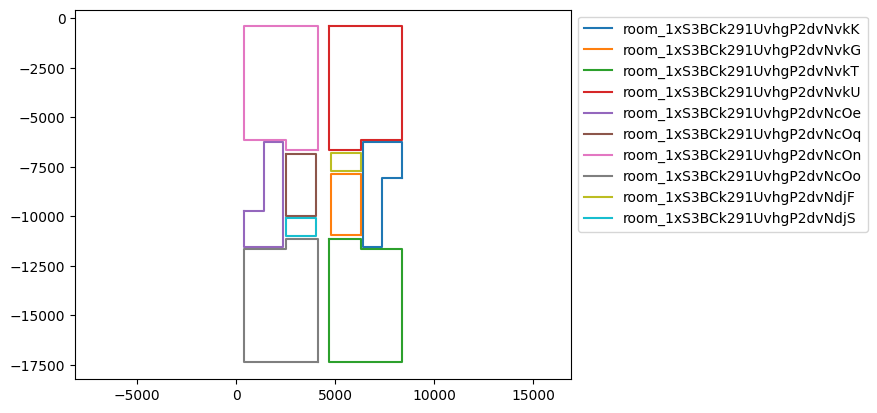
\includegraphics[width=\textwidth]{figures/png/WKT output/output2.png}
\end{figure}

\begin{minted}[bgcolor=white]{output}
inst:level_1xS3BCk291UvhgP2dvNtSE
dict_keys(['room_1xS3BCk291UvhgP2dvNbq0'])
\end{minted}

\begin{figure}[H]
  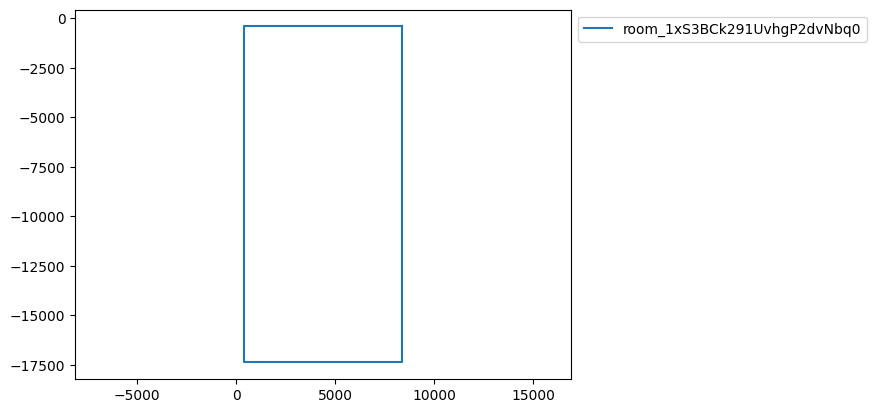
\includegraphics[width=\textwidth]{figures/png/WKT output/output3.png}
\end{figure}

\begin{minted}{python}
def showRoom(level, room):
    polygon = data[level][room]
    plt.figure()
    xs, ys = zip(*polygon)
    plt.plot(xs, ys)
    plt.axis('equal')
    plt.show()
showRoom("inst:level_1xS3BCk291UvhgP2dvNMKI", "room_1xS3BCk291UvhgP2dvNvkw")
\end{minted}

\begin{figure}[H]
  \centering
  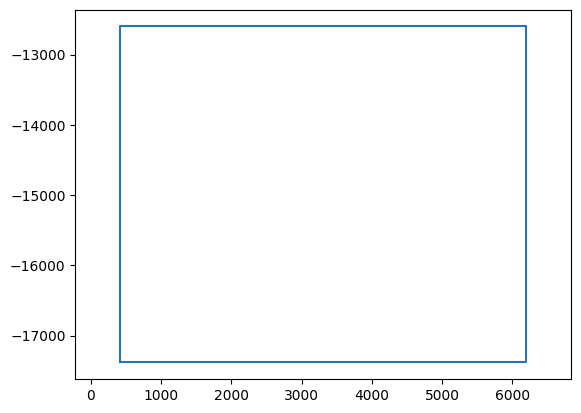
\includegraphics[width=0.7\textwidth]{figures/png/WKT output/output4.png}
\end{figure}

\section{Geometry extraction}
\label{sec:pyhtonExtraction}
\begin{minted}{python}
  import rdflib
  
  g = rdflib.Graph()
  qres = g.query("""
  PREFIX props: <https://w3id.org/props#>
  PREFIX rdf: <http://www.w3.org/1999/02/22-rdf-syntax-ns#>
  PREFIX bot: <https://w3id.org/bot#>
  PREFIX fog: <https://w3id.org/fog#>
  PREFIX xsd: <http://www.w3.org/2001/XMLSchema#>
  SELECT ?s ?o
  WHERE {
    SERVICE <http://localhost:7200/repositories/duplex-v1> {
      ?s fog:asObj ?o .
      filter(datatype(?o)=xsd:string)
    }
  }
  # LIMIT 10
  """)
  
  for row in qres:
      name = row.s.replace("https://172.16.10.122:8080/projects/1001/", "")
      name = name.replace("%", "-") # for github user content
      extention = ".obj"
      directory = "out/"
      fileName = directory + name + extention
      file = open(fileName, "w")
      file.write(row.o)
      file.close()
  \end{minted}

\end{document}
